\documentclass[ 12pt,a4paper,twocolumn,fleqn]{article}
\usepackage{graphicx}
\usepackage[a4paper,top=30mm, bottom=30mm, left=20mm, right=35mm]{geometry}
\usepackage{fancyhdr}
\usepackage{hyperref}
\usepackage{listings}
\usepackage[]{algorithm2e}
\usepackage{color}
\usepackage{fancybox}
\pagestyle{fancy}
\usepackage{lineno}
\usepackage{xtab,booktabs}
\usepackage{setspace}
\usepackage{changepage}
\usepackage{amsmath}
\usepackage{xcolor}
\usepackage[compact]{titlesec}
\usepackage{chngcntr}

\titlespacing{\section}{0pt}{*0}{*0}
\titlespacing{\subsection}{0pt}{*0}{*0}
\titlespacing{\subsubsection}{0pt}{*0}{*0}
\setlength\columnsep{25pt}
\makeatletter
\g@addto@macro{\normalsize}{%
\setlength{\abovedisplayskip}{0pt}
\setlength{\abovedisplayshortskip}{0pt}
\setlength{\belowdisplayskip}{0pt}
\setlength{\belowdisplayshortskip}{0pt}}
\makeatother
\mathindent=0.0pt
\usepackage{float}
\renewcommand{\baselinestretch}{1.5}
\begin{document}
\pagenumbering{gobble}
\lhead{Computer Vision Based CCTV Accident Detection}
\chead{}
\rhead{Batch 2}
\onecolumn


\newpage
  \pagestyle{fancy}
\tableofcontents

\newpage
  \pagestyle{fancy}
\listoffigures

\newpage
  \pagestyle{fancy}
\begin{adjustwidth}{3.5em}{0pt}
\pagenumbering{arabic}
\setcounter{page}{1}
\section{Introduction}
\subsection{The Problem}

The 2000’s have seen a massive rise in vehicle ownership across the World. This has also had a direct effect on the rise of road accidents in the same timeframe. What is worrying is that the casualties of these road accidents have also been on the rise year-on-year. Various factors play a role in the low survival rates of accident victims, one of the most important ones being the time taken for crucial medical aid to be administered. The total time taken for this first aid to reach the victim can be divided into two segments, T1 and T2.

\begin{figure}[h]
    \centering
    \hspace*{0.4in}
    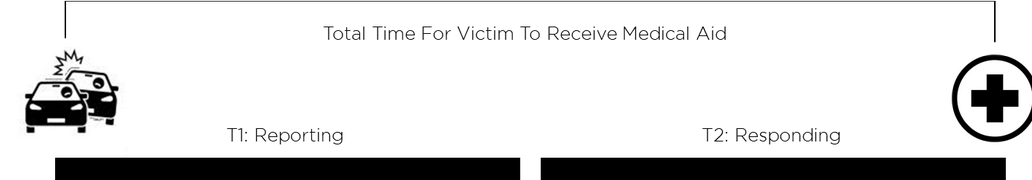
\includegraphics[scale=0.4]{media/t1.png}
    \caption{Emergency Response (Time Breakdown)}
    \label{fig:my_label}
\end{figure}

T1 - Reporting:
T1 is the time between the accident occurring and it being reported to the nearest emergency center or hospital. This is the segment that has the most variation, as for an accident to be reported, there must be someone present at the scene of the accident to manually inform the center that the accident had occurred. Certain modern car models are fitted with sensor arrays and systems that report these accidents, but the vast majority of vehicles across the country and the world are not equipped with these services. 

T2 - Responding:
T2 is the time between the accident being reported and the medical aid reaching the victim. This segment is more controlled, with efficient systems in place that dispatches medical aid quickly. The only hurdles faced in this segment are the ones that cannot be controlled, such as weather conditions, road traffic and so on.

The sum total of both these segments should be under an hour, in order for the victim to have the best possible chances
of survival. From the above descriptions, we see that the segment with the best chance of improvement is the time taken for the accident to be reported or T1. Our goal is to minimize this, by automatically detecting accidents through the CCTV camera network that already exists, and allowing emergency care centers to instantly dispatch medical aid. This gives the victim the best possible chance to receive care in the golden hour, maximizing their chances of survival.


\hspace{0.2cm}



\subsection{Real World Application}
The project was designed to solve a real problem and be applied in the real world. By leveraging the existing CCTV Camera network, we reduce our hardware dependencies. Some of the most noteworthy real world applications are :
\begin{enumerate}

  \item {Victims of Road Accidents get emergency care quickly
The first main application is that victims of road accidents get access to emergency care in a timely manner. By eliminating the time it takes to report the accident, we give the victim the best possible chance of survival by directly reporting and notifying the nearest emergency care center of the occurrence of the accident.}

  \item {Quick resolution of potential roadblocks and traffic blockades
Another application of the project is the quick resolution of traffic blockades. By efficiently reporting the occurrence of an accident to traffic monitoring centers, police personnel can be dispatched to guide vehicular movement in the vicinity of the accident to ensure the smooth flow of traffic.}

\item {Efficient utilization of emergency resources
The project would also ensure that emergency resources are efficiently utilized, by dispatching the accident details to the closest emergency response center. The image of the accident also ensures the center can take the best decision on the resources required to take care of the accident, without having to guess the resources require}
\end{enumerate}

\newpage
  \pagestyle{fancy}
  
\subsection{Organisation of Project Report}

The project report is organized as follows:\\
In Chapter (2) we discuss the problem statement and the proposed solution. We also take a look at the systems that exist today and the drawbacks they face. \\
Chapter (3) takes a more in-depth look at various hardware and software based solutions that exist, with a survey on existing literature available. \\ Chapter (4) looks at the architecture of the proposed solution with an overview of the system design, utilizing system block diagrams and data flow diagrams. \\
Chapter (5) dives into the Implementation of the solution, by describing the hardware and software requirements, along with dataset descriptions and implementation details. \\
Chapter (6) describes our testing process, while Chapter (7) looks at our experimentation process and the obtained results. \\
Chapter (8) summarizes our findings and concludes the paper. 


\newpage
  \pagestyle{fancy}
\section{Problem Statement and Proposed Solution}
\subsection{Problem Statement}

To develop and detect accidents efficiently and accurately from CCTV camera footage.


\hspace{0.2cm}


\subsection{Existing Systems}

Numerous solutions have been put forth to tackle detection of accidents. Some solutions make use of existing sensors in vehicles or in road junctions to detect various parameters that may indicate a potential accident. These sensors keep an eye on the speed, vibration etc. of the vehicle and report accidents in case of anomalous values. Solutions which make use of sensors in the vehicles also have mechanisms to stop the motion of the vehicle in case of unexpected values. Other solutions analyze video frames in order to figure out if an accident has occurred.

\hspace{0.2cm}


\subsubsection{Deep Learning and Computer Vision based systems}
In terms of detecting accidents using Computer Vision, Ali Pashai came up with an efficient method of using Convolutional Neural Networks to classify accidents based on their type and severity. By leveraging various other deep learning techniques, several other works were published regarding classification and detection of accidents. A highly helpful approach that takes into account the many visual characteristics of an accident incident was proposed by Robles-Serrano. in 2021. This particular work shows the superiority of Convolutional Neural Networks in comparison to other deep learning based approaches.

\hspace{0.2cm}

According to S. Ghosh, the ability of CNN to perform feature extraction in combination with a binary classifier can be used to detect accidents on their own as well. However, this introduces a larger margin for error depending on the kind of images that the network acts on, the proportion of features that are related to accidents, and other factors.

\hspace{0.2cm}


When it comes to locating accidents, feature extraction together with the localisation of the cars involved and their attributes may also be useful. By using object detection to localise the accident site as proposed by Bochkovskiy, we can exclusively concentrate on the cars involved in the collision. This enables for a more precise type of feature extraction to be carried out on the confined region. To calculate the distance between two cars involved in a collision, Earnest Paul Ijjina suggested using centroid tracking approaches in addition to Euclidean distance.

\newpage
 \pagestyle{fancy}
 
\subsection{Proposed Solution}

Combining the various editing methods, we propose a solution that not only makes use of Deep Learning based feature extraction but also takes into consideration the locality of the occurred accident in terms of the entire frame by leveraging state of the art Object Detection methodologies combined with a custom collision detection algorithm.
The approach to accident detection can be classified into two separate stages.
\begin{itemize}
   \item { Detection of Vehicles involved in an accident via object detection and a collision algorithm }
   \item {Classification of the detected accident by the use of two separate CNN and ANN models. }
   \begin{itemize}
       \item Google’s Densenet-201 for primary feature extraction.
       \item A fully connected multi layer neural network.
   \end{itemize}
\end{itemize}


\hspace{0.2cm}



\subsubsection{Object Detection using YOLO}

The first step of the solution involves accurately detecting vehicles in a given frame, we successfully accomplish this in real-time by making use of YOLOv4.

YOLO is an algorithm that provides real-time object detection using neural networks.
The popularity of this algorithm is due to its accuracy and quickness.
It has been applied in a variety of ways to identify objects such as people, animals and vehicles.
Various methods are used for object identification, including Retina-Net, fast R-CNN, and Single-Shot MultiBox Detector (SSD).
These methods have addressed the problems of data scarcity and modelling in object detection, however they cannot find objects in a single algorithm run. Due to its better performance over the aforementioned object identification approaches, the YOLO algorithm has grown in popularity.


\begin{figure}[h]
\begin{center}
    \hspace*{0.4in}
    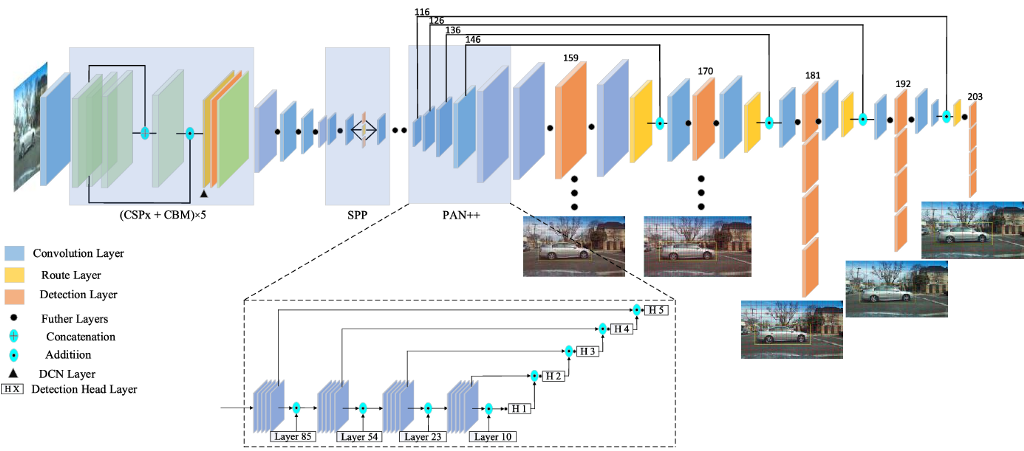
\includegraphics[scale=0.4]{media/yolo_arch.png}
    \centering
  \caption{    YOLO-v4 architecture}
\end{center}
\end{figure}

\hspace{0.2cm}

YOLO works in real-time depending on the hardware used to run it. It takes in an input image and produces an output bounding box which consists of the coordinates in two dimensional space with respect to an image.
In our particular use-case, we made use of YOLO v4 which has better accuracy and efficiency when compared to it’s predecessors. We made use of the pre-trained YOLOv4 model and further trained on 10000 images of cars with their bounding box annotated.

\hspace{0.2cm}

\begin{figure}[H]
\begin{center}
    \hspace*{0.4in}
    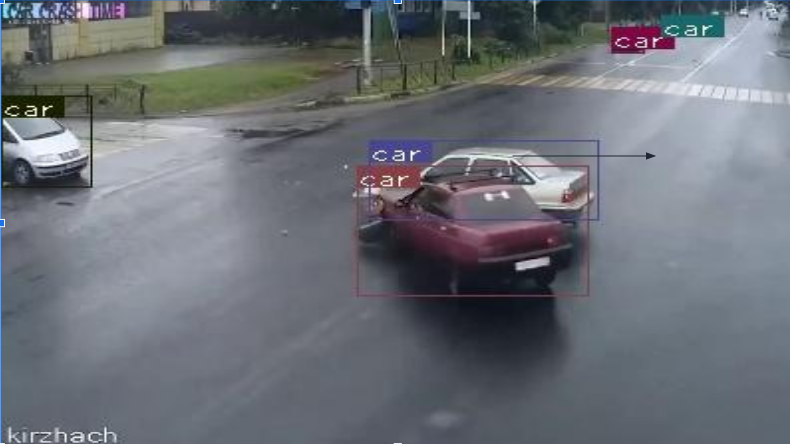
\includegraphics[scale=0.5]{media/yolo.png}
    \\
  \caption{    Working of YoloV4}
\end{center}
\end{figure}

\newpage
 \pagestyle{fancy}



\subsubsection{Collision Detection}
After we detect the vehicles in the frame, we move onto the collision detection step. Our intention is to localise the region where an accident might have happened, instead of attempting to detect the accident on an entire frame. 
The algorithm designed for the same is based on the Axis Aligned Bounding Box(AABB), where the edges of the box are parallel to the Cartesian coordinate axes. We take the bounding boxes of the detected vehicles and their coordinates as used by OpenCV where the origin of the image is located at the upper-left hand corner. We then take the horizontal and vertical distances between the centres of the two detected bounding boxes, and subtract the half widths and half heights of the boxes from them respectively to determine if the boxes overlap. If the resultant value is negative in both cases, we can confirm that the boxes overlap, and there might be an accident.

\hspace{0.2cm}

\begin{figure}[H]
\begin{center}
    \hspace*{0.4in}
    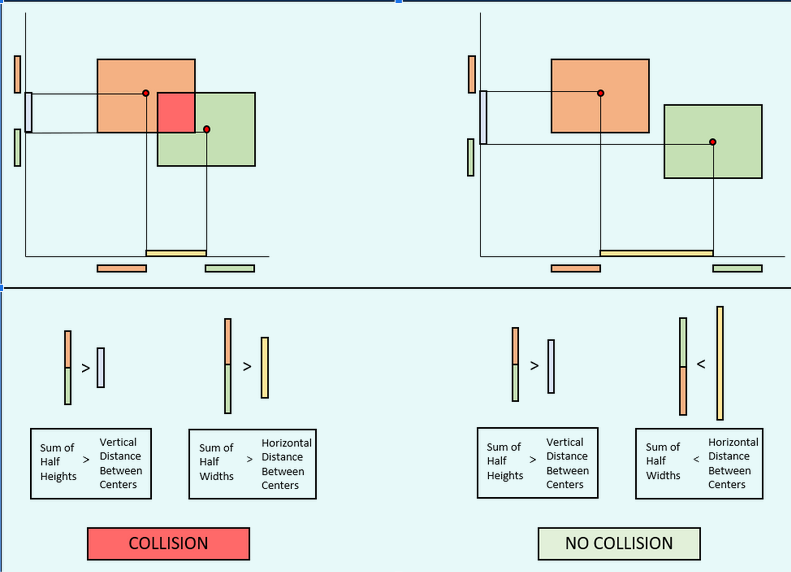
\includegraphics[scale=0.4]{media/coll.png}
    \\
    \centering
  \caption{ Axis Aligned Bounding Box Collision Detection Algorithm}
\end{center}
\end{figure}

However, to counter an irregularity in the object detection process where two vehicles, on impact, are detected as a single object as seen in the figure below, we check if the resultant values are less than 5\% of the half width and height, to allow the algorithm to shortlist cases where the vehicles are about to collide. 
\hspace{0.2cm}
As this algorithm only involves checking ranges of coordinate values, it is computationally less intensive than other approaches such as Intersection over Union, and this also allows us to quickly eliminate objects that are far apart in the frame, allowing us to process situations with multiple objects in the frame quickly.

\hspace{0.2cm}


\subsubsection{Feature Extraction using Densenet-201 and Classification}

After we detect a possible accident using the collision detection algorithm, we crop the region of the image where the collision was detected and is sent to a classifier that predicts the probability that an accident has occurred in that region. By doing so, we minimise cases where cars pass close by each other but do not necessarily collide.

\hspace{0.2cm}

Ali Pashaie et al have established an image based approach for classification of accidents which takes the entire image for feature extraction and classification but doing so in situations where the accident occurs in a small region of the image results in the accidents being ignored. By taking only the region where an accident might have happened, we significantly increase the probability of correctly predicting the accident.

\hspace{0.2cm}

Feature extraction can be formally defined as : The dimensionality reduction method, which divides and condenses a starting set of raw data into smaller, easier-to-manage groupings.
This causes the resulting processing to be a lot simpler as we deal with much smaller dimensions. The fact that these enormous data sets contain a lot of different variables is their most crucial feature and processing these variables takes a lot of computational power.
In order to efficiently reduce the amount of data, feature extraction helps to extract the best feature from such large data sets by choosing and combining variables into features.
\hspace{0.2cm}

The way CNN operates is to obtain an image, assign it a weight depending on the various items in the image, and then separate them from one another. In comparison to other deep learning algorithms, CNN requires extremely minimal pre-processing of the input.
\hspace{0.2cm}

The working of a Convolutional Neural Network can be split into 3 separate layers

i) The first layer is the Convolutional Layer, which is the central component and handles the majority of the computational labour, is the first layer in a CNN network.
Filters or kernels are used to convolute data or images.

ii) The Second Layer is the Activation Layer which introduces non-linearity in the CNN

iii) The Third layer is the Pooling Layer which essentially down samples the features obtained in the previous layers.

This entire procedure is repeated multiple times to gather features from the specified input image.

\begin{figure}[H]
\begin{center}
    \hspace*{0.4in}
    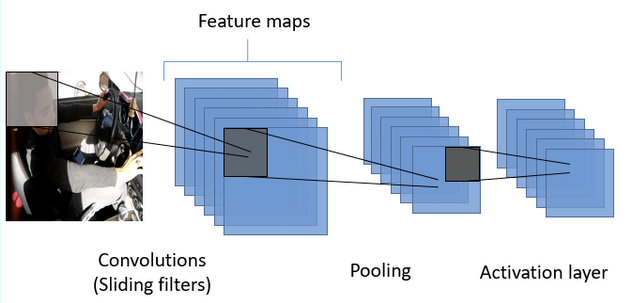
\includegraphics[scale=0.6]{media/conv.png}
    \\
  \caption{    Working of CNN}
\end{center}
\end{figure}
% cnn image (cat)

Instead of beginning from scratch to solve an issue that is similar, we utilise a model that has already been trained on images that are similar to our use-case or general images. This essentially allows us to re-use a pre-trained model without having to worry about how or if the CNN is learning specific features.

As CNN’s become increasingly deep, information about the input passes through many layers and the gradient of the loss function approaches zero, causing it to vanish by the time it reaches the end of the network. In standard ConvNets, the input image goes through multiple convolutions to obtain high-level features. In ResNet, element wise addition is used where the previous layer is merged additively into the future layer which forces the network to learn errors in between the previous layers and the current one.

\hspace{0.2cm}
DenseNet-201 is a Convolutional Neural Network that has 201 layers where each layer obtains inputs from all preceding layers and passes its own feature maps to the subsequent layers where it focuses on concatenating the outputs from the previous layers instead of using a summation. Since each layer receives feature maps from the preceding layers, the network can be thinner and more compact. This helps achieve higher computational and memory efficiency.

\begin{figure}[H]
\begin{center}
    \hspace*{0.4in}
    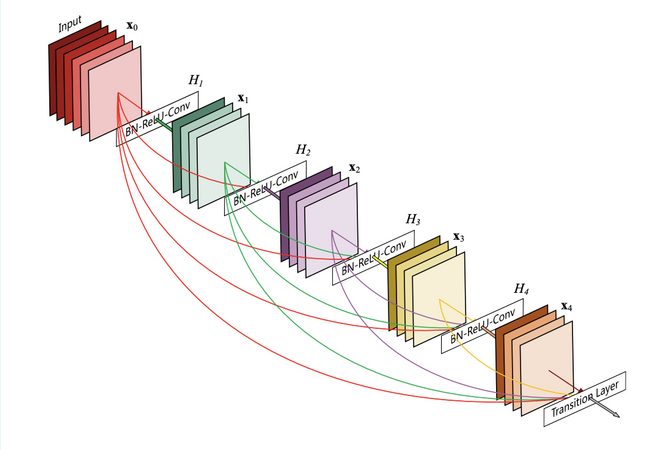
\includegraphics[scale=0.4]{media/dense.png}
    \\
    \centering
  \caption{    Working of Densenet-201}
\end{center}
\end{figure}
% add densenet image

A Dense Block is a module that directly links all layers (with corresponding feature-map sizes).
Concatenating feature maps learned by different layers increases variation in the input of subsequent layers and also improves efficiency. This constitutes a major difference between DenseNets and ResNets. Compared to Inception networks, which also concatenate features from different layers, DenseNets are simpler and more efficient. 
\hspace{0.2cm}

DenseNet is much more efficient in terms of parameters and computation for the same level of accuracy when compared with ResNet, both networks having been trained and classified on the Imagenet validation set results.

\hspace{0.2cm}

Feature extraction being performed by the Densenet-201 model produces a feature vector of shape (1,1920) which on flattening gives a vector of (1920,). Each image is resized to 224x224x3 pixels which is then resized to (1,224,224,3) which is the input format required by Densenet-201.

\begin{figure}[H]
\begin{center}
    \hspace*{0.4in}
    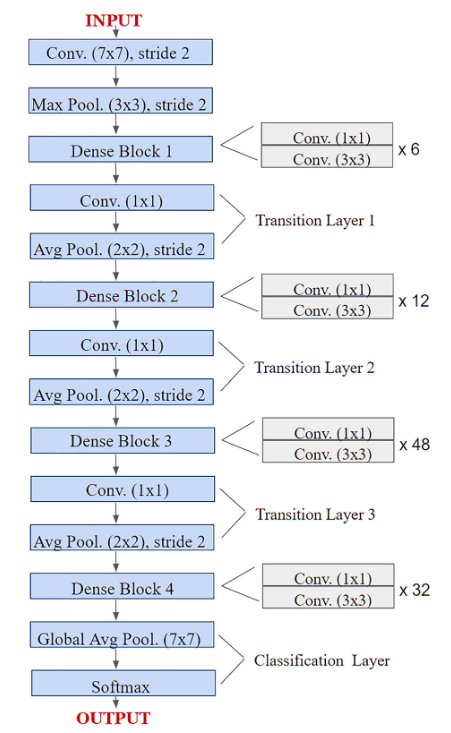
\includegraphics[scale=0.7]{media/dense_arch.png}
    \\
    \centering
  \caption{ Densenet 201 Architecture}
\end{center}
\end{figure}


\newpage
  \pagestyle{fancy}

\subsection{Neural Network following the Feature Extraction}
After the extraction of features, these features are then fed to an Artificial Neural Network which then handles the task of accident classification. The output of the Densenet-201 model produces a vector of length 1920 which basically contains the required features of the input image.This (1920,1) dimension vector is fed to a Neural Network with an input layer od 16 neurons, followed by two hidden layers of 32 and 16 neurons each and a final output layer.

\hspace{0.2cm}

Between each layer, there exists a dropout layer to prevent over-fitting, a Rectified Linear Unit (ReLU) and a Sigmoid activation function between the last hidden layer and the output layer.

\begin{figure}[H]
\begin{center}
    \hspace*{0.4in}
    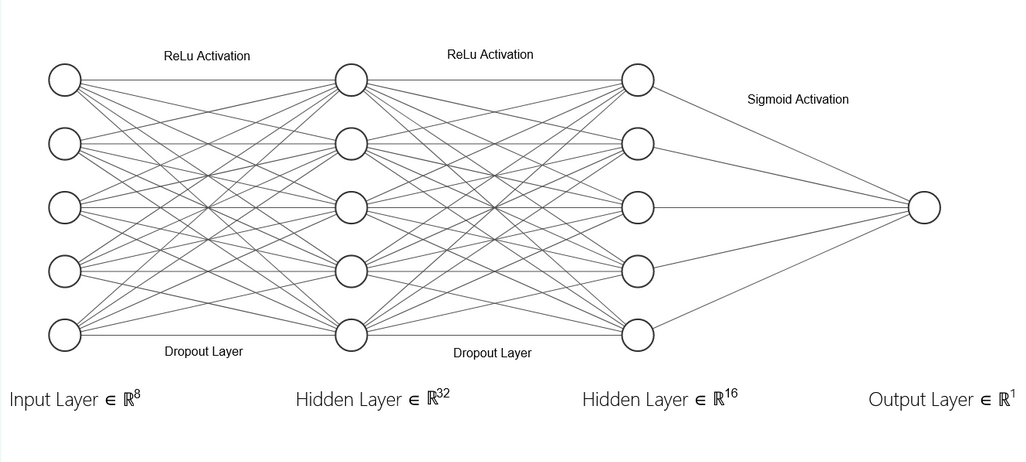
\includegraphics[scale=0.4]{media/ann.png}
    \centering
    \\
  \caption{ Neural Network Architecture}
\end{center}
\end{figure}

Having a single output neuron would allow for the specification for minimising false positive cases. In our case we set the threshold to be ~0.82, this causes all of the accidents with probability \> 0.82 to be classified as an accident.


\hspace{0.2cm}


\subsection{System Requirements}
\begin{itemize}
    \item Processor : min processor required
    \item Memory : Minimum of 16 GB ram for computation
    \item Video Memory : Minimum of 3 GB of VRAM for Object Detection and another 2 GB for feature extraction and the ANN.
\end{itemize}

\newpage
  \pagestyle{fancy}

\section{Literature Survey}

Numerous solutions exist to detect accidents. They can broadly be divided into two categories :
\begin{itemize}
    \item Hardware solutions
    \item Software solutions
\end{itemize}
Hardware solutions tackle the detection process primarily through sensors attached to vehicles or through the ones that are present at junctions. On the other hand, software solutions analyze video feeds to decide if an accident has occurred. The following subsections talk about various hardware  and software solutions in detail.

\hspace{0.2cm}


\subsection{Hardware solutions}

\hspace{0.2cm}


\subsubsection{IOT Based Automatic Accident Detection And Rescue Management In Vanet}

Authors: Manuja M, Kowshika S, Narmatha S, and Gracy Theresa W

This paper handles accident detection and reporting by making use of Vehicular Ad-hoc networks (VANETs). In VANETs, a moving vehicle is considered to be a node and thus, a group of vehicles are able to communicate with each other. Vehicles, on sensing an accident using their built-in sensors, relay the alert messages using their RF modules. Since messages are being communicated using RF modules, a nearby moving vehicle, which is in the range of the RF module can pick this message up and transport it to another vehicle and so on, until the message reaches a vehicle that is in the network of the Road Side Units (RSUs). Finally, the message is passed on to the base station (RSU). This work around where we use RF modules instead of GSM modules proves to be pretty helpful for areas where the vehicles are not in the network of RSUs.  



\hspace{0.2cm}

\subsubsection{Development of Message Queuing Telemetry Transport (MQTT) based Vehicle Accident Notification System}

Authors: Bharat Naresh Bansal and Vivek Garg

Description: The prototype presented in this paper is an accident notification system using an ESP8266 NodeMCU, and its central component is a simple vibration sensor. The vibration sensor continuously detects vibrations, and when they reach a certain threshold limit, it notifies the registered phone numbers. Similar models have previously been proposed, but they used more expensive sensors like accelerometers. The concept in this work, however, uses a simpler and less expensive sensor. Earlier versions employed GSM technology, but the suggested concept  employs a Wi-Fi based controller, which is more dependable and quick than GSM technology. The usage of NodeMCU eliminates the need for any other controller, which was also necessary for older GSM modules, which required an additional microcontroller such an Arduino. The prototype system described in this study uses the message queuing
telemetry transport (MQTT) protocol which is very dependable. Adafruit IO, an IoT cloud platform, is used in this prototype and is much easier to use than other IoT cloud platforms like Losant Platform. Additionally, Adafruit IO updates its data every two seconds. IFTTT and ClickSend platforms are used for the protocol's notification purposes, and Applets and Triggers are developed to meet the demand.


\hspace{0.2cm}

\subsubsection{An IoT based car accident prevention and detection system with smart brake control}

Authors: Mubashir Murshed and Md Sanaullah Chowdhury
 
Description:This paper describes a smart system that alerts and controls the speed of the vehicle. It also notifies individuals in the event of an accident.Using a distance sensor, this system continuously keeps track of the distance between the vehicles and any impediments in front. When a critical distance approaches, it will warn the driver to regulate speed and automatically slow down. An email alert with the car's information will be sent to the accountable person whenever an accident occurs.


\hspace{0.2cm}

\subsection{Software Solutions}

\subsubsection{Automatic Detection of Traffic Accidents from Video Using Deep Learning Techniques}

Authors: Sergio Robles-Serrano, German Sanchez-Torres, and John Branch-Bedoya

Description:  Approaches based on deep learning (DL) have demonstrated strong performance in computer vision challenges involving complicated feature relationships. In this paper, a video-based automatic DL-based approach for traffic accident detection has been developed. The model architecture is composed of an extraction step for visual features and a subsequent phase for temporary pattern detection. Convolution and recurrent layers are used in the training phase to learn the visual and temporal features from scratch. In public traffic accident datasets, an accuracy of 98 percent is attained in the detection of accidents, demonstrating a strong capacity in detection independent of the road structure.


\hspace{0.2cm}

\subsubsection{Convolution neural network joint with mixture of extreme learning machines for feature extraction and classification of accident images}

Authors: Ali Pashaei, Mehdi Ghatee, and Hedieh Sajedi

Description: This paper detects accidents from images. The method proposed can be divided into two stages. The first stage consists of the feature extraction process for which a deep learning method has been developed. Hidden features are extracted from the last max-pooling layer of a Convolution Neural Network (CNN). The next stage deals with classification. For this, a combination of advanced variations of Extreme Learning Machine (ELM) -
1. basic ELM
2. constraint ELM (CELM)
3. On-Line Sequential ELM (OSELM) 
4. Kernel ELM (KELM)


\hspace{0.2cm}

\subsubsection{Accident Detection Using Convolutional Neural Networks}

Authors:  Sreyan Ghosh, Sherwin Joseph Sunny and Rohan Roney

Description: The cause of more than 80\% of accident-related fatalities is not the accident itself but rather the failure to provide prompt aid to accident victims. An accident victim could be left unattended for a very long time on highways, where traffic is extremely light and moving quickly. The goal is to develop a system that can recognise an accident based on a live video feed from a CCTV camera mounted on a highway. Each frame of a video will be passed through a deep learning convolution neural network model that has been trained to distinguish between accident and non-accident related video frames. It has been demonstrated that Convolutional Neural Networks provide a quick and reliable method for classifying photos. For comparatively smaller datasets, CNN-based image classifiers have achieved accuracy levels of above 95\% and need less preparation than other image classification algorithms.


The combination of advantages of the above ELMs have made it possible for this method to provide highly accurate results along with a near real-time processing speed.

\newpage
  \pagestyle{fancy}
  
 \section{Architecture and System Design}
 
The overview of the system is represented in Fig.4.1. It shows the modules involved in building the system i.e,

\begin{itemize}
    \item CCTV camera
    \item A Server
    \item Google Firebase real-time database
    \item Web -User Interface
\end{itemize}

\newpage
  \pagestyle{fancy}
  
\subsection{Software Overview}

\subsubsection{System Block Diagram}

\begin{figure}[H]
\begin{center}
    \hspace*{0.4in}
    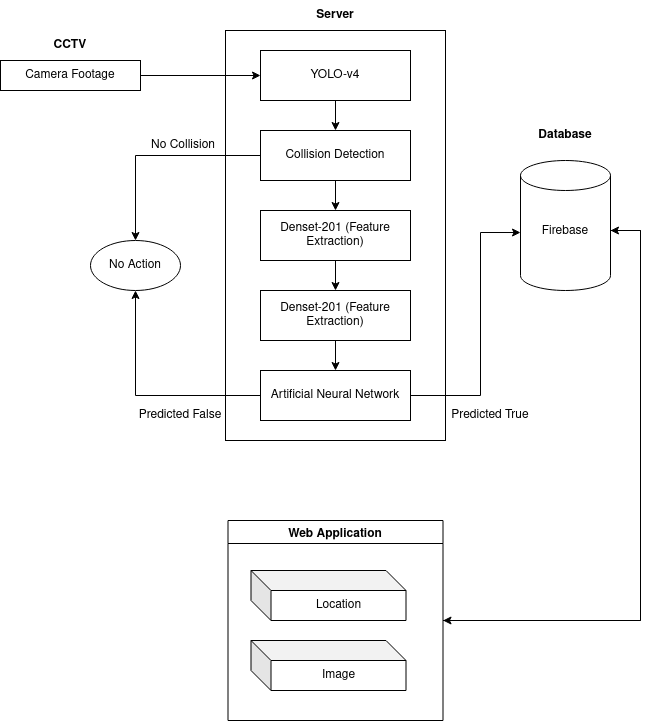
\includegraphics[scale=0.6]{media/system_block.png}
    \centering
    \\
  \caption{ System Block Diagram}
\end{center}
\end{figure}

\newpage
  \pagestyle{fancy}

CCTV footage from multiple cameras is first streamed into a server. This server runs the Accident detection application, which analyses the stream and gives a prediction of True or False in real time. If an accident is detected at any instance, a single frame in which the accident was predicted is cropped, bundled with metadata such as location and time of the accident and sent to the Firebase database. 
The front-end Web User Interface which is built using Vue.js is continuously watching the Firebase database and automatically updates the client view as soon as the data is written to the database.

\hspace{0.2cm}

\subsubsection{Data Flow Diagram}
\begin{figure}[H]
\begin{center}
    \hspace*{0.4in}
    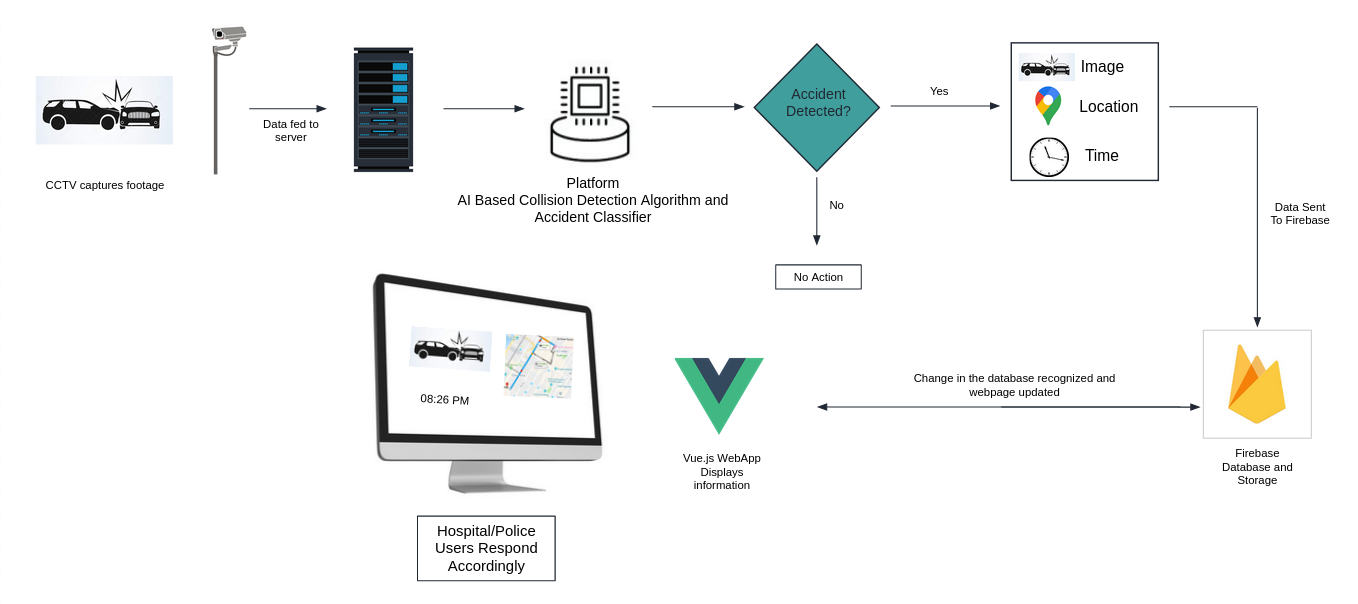
\includegraphics[scale=0.3]{media/arch.png}
    \centering
    \\
  \caption{ Data Flow Diagram}
\end{center}
\end{figure}

\begin{itemize}
    \item First vehicle detection is run on the video stream from the CCTV footage, this gives the bounding boxes of each vehicle in the view of the camera.
    \item With the collision detect algorithm discussed in earlier sections, a frame of the image is predicted to have a collision or not.
    If prediction is True, the frame is passed into the Artificial Neural Network also described earlier.
    \item Artificial Neural Network predicts true or false.
    \item In the case the prediction is false, No action is taken and the next frame is analysed.
    \item Otherwise, the frame is uploaded to google Firebase block storage and metadata such as image URL, Longitude, Latitude and Timestamp is appended to the Firebase Firestore database.
    \item Data is automatically fetched and displayed on the Web UI. 
\end{itemize}



\newpage
  \pagestyle{fancy}
  
 \section{Implementation}
 
 \subsection{Implementation Platform}
 
 \subsubsection{Hardware}
 
  i) Processor: AMD Ryzen 5 3600 4.2Ghz 6 cores 12 threads
 
 ii) RAM: 16GB DDR4 3533 MT/s
 
 iii) GPU: Nvidia GeForce RTX 3070 8GB
 
 iv) Storage platform: NVME SSD
 
 
 \subsubsection{Software} 
 i) Operating System: Linux 64bit (Docker container)
 
 ii) Software Used : TensorFlow, OpenCV, Darknet, Vue.js 2.0, Firebase
 
 iii) Programming Languages : Python 3, Javascript
 
 iv) Server: Python HTTP server
 
 
 \newpage
  \pagestyle{fancy}
 
\subsection{Implementation Details} 

\subsubsection{Organisation of files}

\begin{figure}[H]
\begin{center}
    \hspace*{0.4in}
    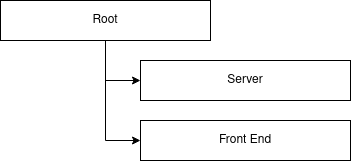
\includegraphics[scale=0.6]{media/root.png}
    \\
  \caption{ Root directory structure  }
\end{center}
\end{figure}

\hspace{0.2cm}

\begin{figure}[H]
\begin{center}
    \hspace*{0.4in}
    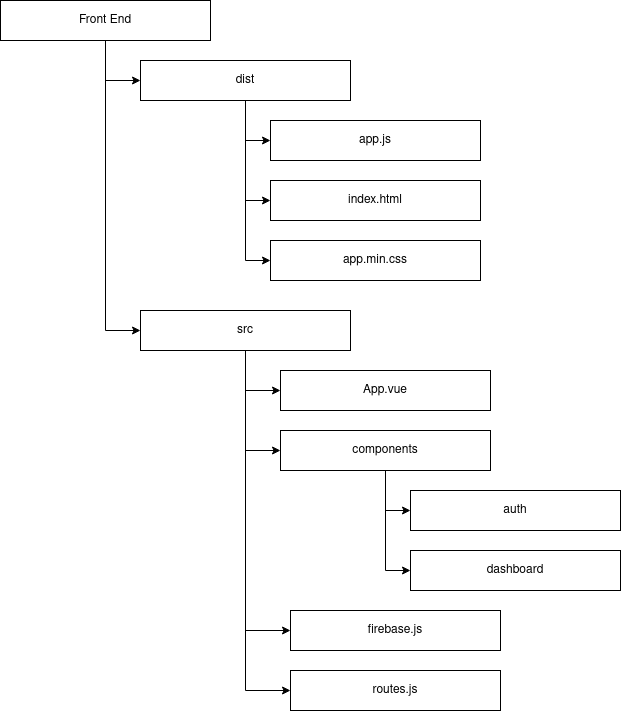
\includegraphics[scale=0.6]{media/frontend.png}
    \\
  \caption{ Front End directory structure}
\end{center}
\end{figure}

\hspace{0.2cm}

\begin{figure}[H]
\begin{center}
    \hspace*{0.4in}
    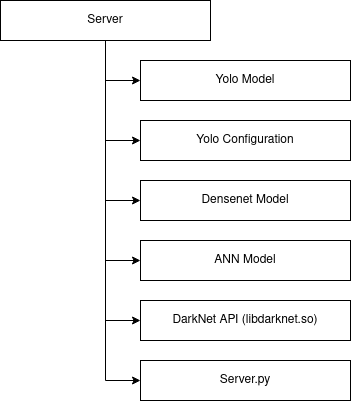
\includegraphics[scale=0.6]{media/backend.png}
    \\
  \caption{ Server directory structure}
\end{center}
\end{figure}

The project consists of two services, the back-end accident detection framework which is run on a server and a client viewable front end. The Firebase database acts as a mediator between the two. As a result, both can be run and hosted independent of each other. Server can be hosted on a powerful machine and the front end can be hosted on any static web hosting service. There are 2 main folders, Server and Web. 

\hspace{0.2cm}

As the name suggests, server contains all the necessary files for detecting the accident, which include the YOLO model, configuration for YOLO model, the Densenet model, the Ann model and the core logic itself for detecting accidents in main.py. The web user interface folder consists of 2 sub folders - dist and src. Dist contains the minified and compressed HTML and JS, which is meant and optimised for deployment. The src folder contains the structure of the front-end which contains the code for all the routes such as login, dashboard, history and location settings.

\newpage
  \pagestyle{fancy}
  
\subsubsection{Implementation Workflow}

The entire process can be defined as per the following 5 step workflow.

\begin{figure}[H]
\begin{center}
    \hspace*{0.4in}
    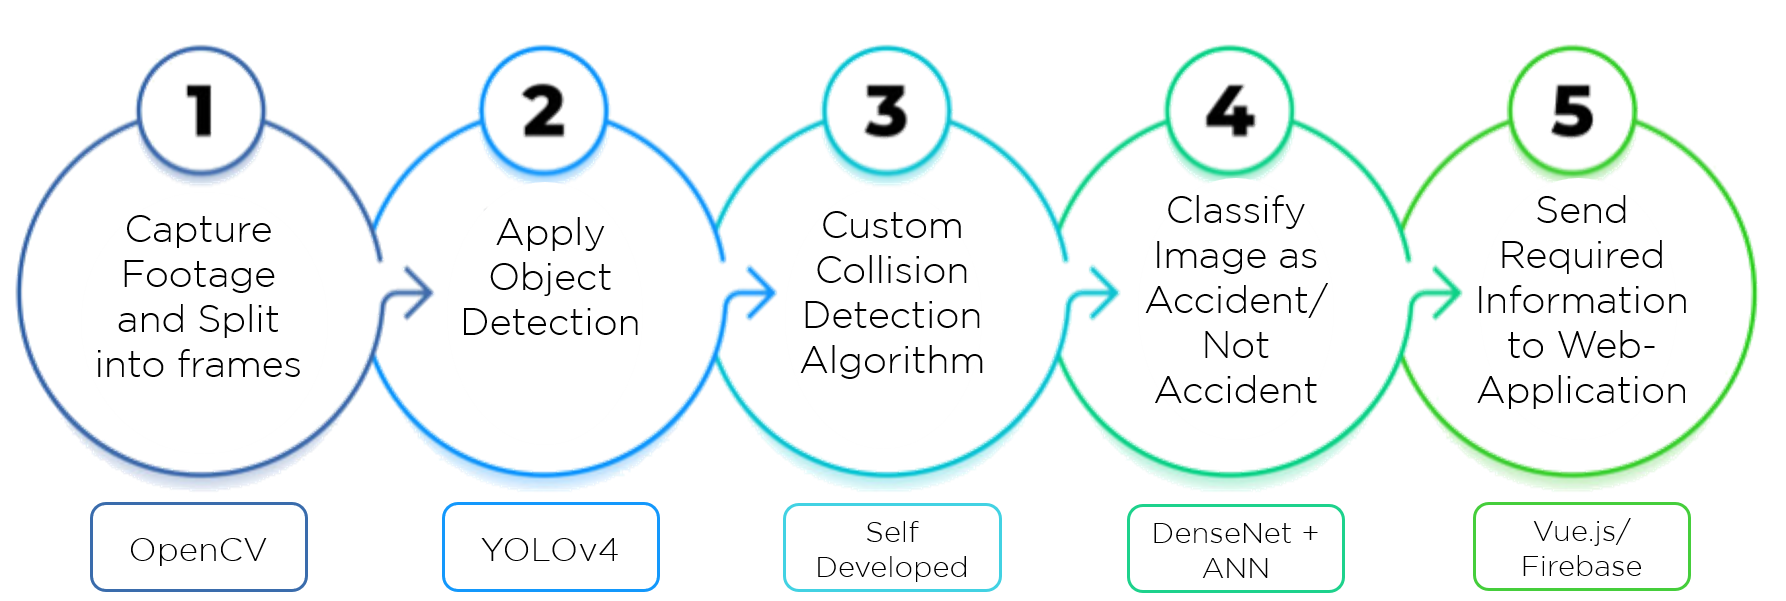
\includegraphics[scale=0.3]{media/flow.png}
    \\
  \caption{ Step-wise Implementation  }
\end{center}
\end{figure}

\begin{itemize}
    \item {Stage 1: Frame Extraction
The first step involves the extraction of the frames from the input video. The video stream is divided down into its constituent frames, which are individually taken and used for processing to detect potential collisions and accidents.}

    \item{Stage 2: Object Detection
The second step acts on the frames that come out the previous step. It's also the first level of processing performed on each frame. For the same, we use You Only Look Once (YOLOv4).
YOLO detects the different objects in each frame, and stores their bounding boxes. For the purpose of this project, we leverage YOLO's ability to detect care, trucks, bikes and other vehicle classes. At the end of this step, we are left with the bounding boxes of all the vehicles in each frame.}
    \item{Stage 3: Collision Detection
The third step in the process is to detect potential collisions in the frame. For the same, we have created a custom collisions detection algorithm based on the Axis Aligned Bounding Boxes (AABB) algorithm. We use the bounding boxes generated from the previous step to check for an overlap between different vehicles. If we do detect an overlap, we take the region around the potential collision, crop it and pass it to the next stage of the process.}
    \item{Stage 4: Accident Classification 
The fourth stage of the process is the classification of the region cropped from the previous step. We pass the cropped region through a DenseNet-201 based feature extractor along with a custom ANN that will output an accident score between 0 and 1. If this score is above a set threshold value, we classify the image as an accident. If it falls below the given threshold, we classify it as not an accident. Based on this classification, we proceed with the final step.}
\item{Stage 5: Reporting
The final step in the process is the reporting of these accidents. We use a self developed web dashboard that would be made available to emergency response centers, hospitals and police stations. If the classifier predicts that an accident has occurred, we take the image along with accident metadata like location of the incident and time of the incident and pass it to the platform, that would then display the details. Based on the location and the availability of response resources, the emergency care centers can dispatch the required resources to the scene of the accident, giving the victim the best possible chance of survival.
}
\end{itemize}

\newpage
  \pagestyle{fancy}

\vspace*{\fill}
\begin{figure}[H]
\begin{center}
    \hspace*{0.4in}
    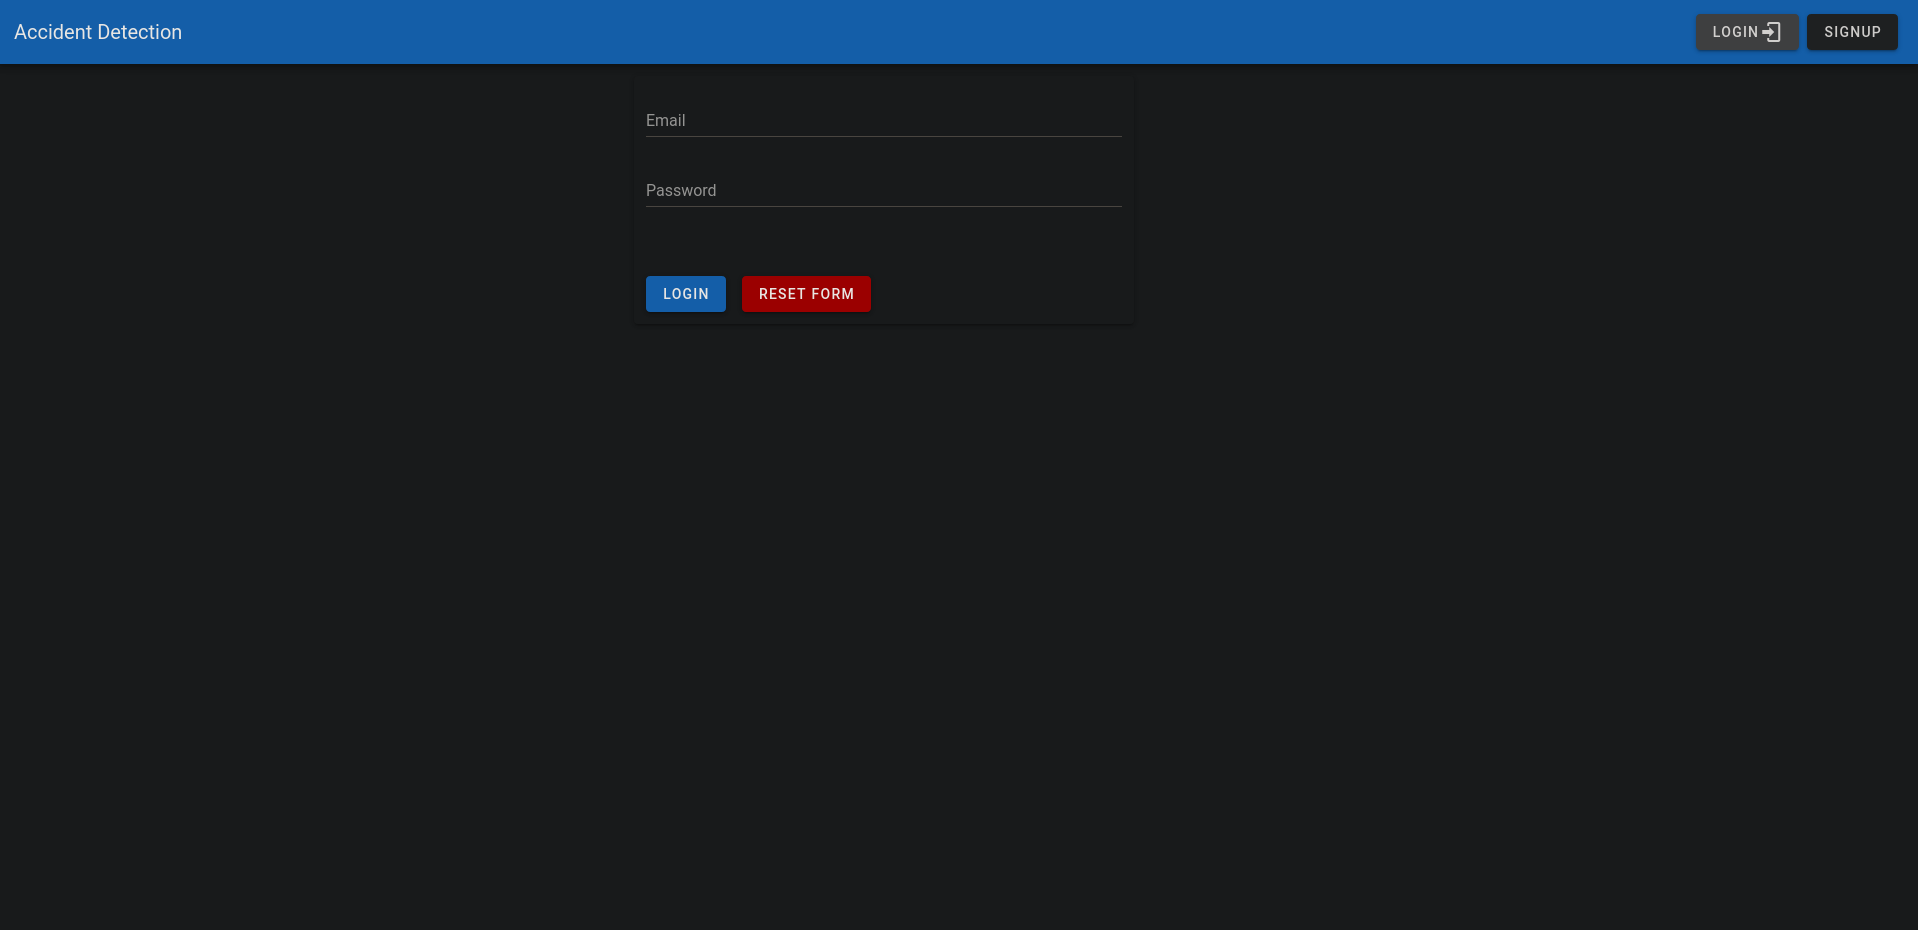
\includegraphics[scale=0.2]{media/login.png}
    \\
  \caption{ Login for Dashboard }
    
\end{center}
\end{figure}

\begin{figure}[H]
\begin{center}
    \hspace{0.2cm}
    
    \hspace*{0.4in}
    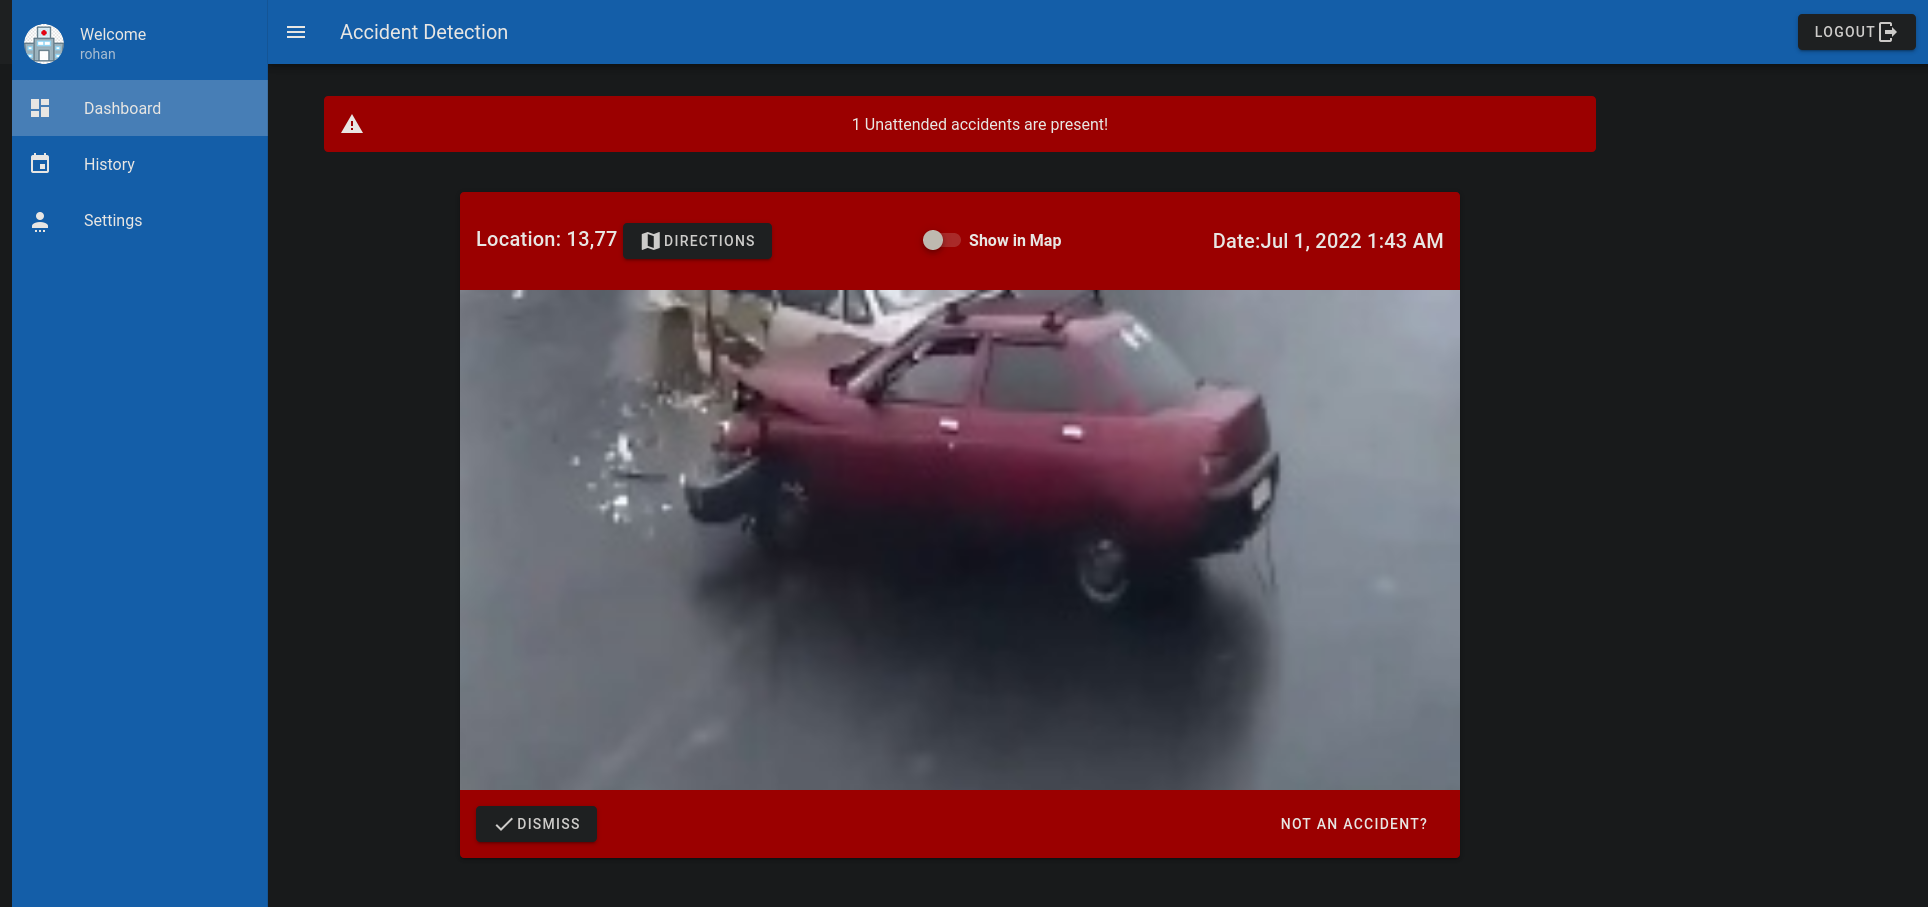
\includegraphics[scale=0.2]{media/ui1.png}
    \\
  \caption{ Reporting Dashboard}
    
\end{center}
\end{figure}
\vfill 

\newpage
  \pagestyle{fancy}

\vspace*{\fill}
\begin{figure}[H]
\begin{center}
    \hspace*{0.4in}
    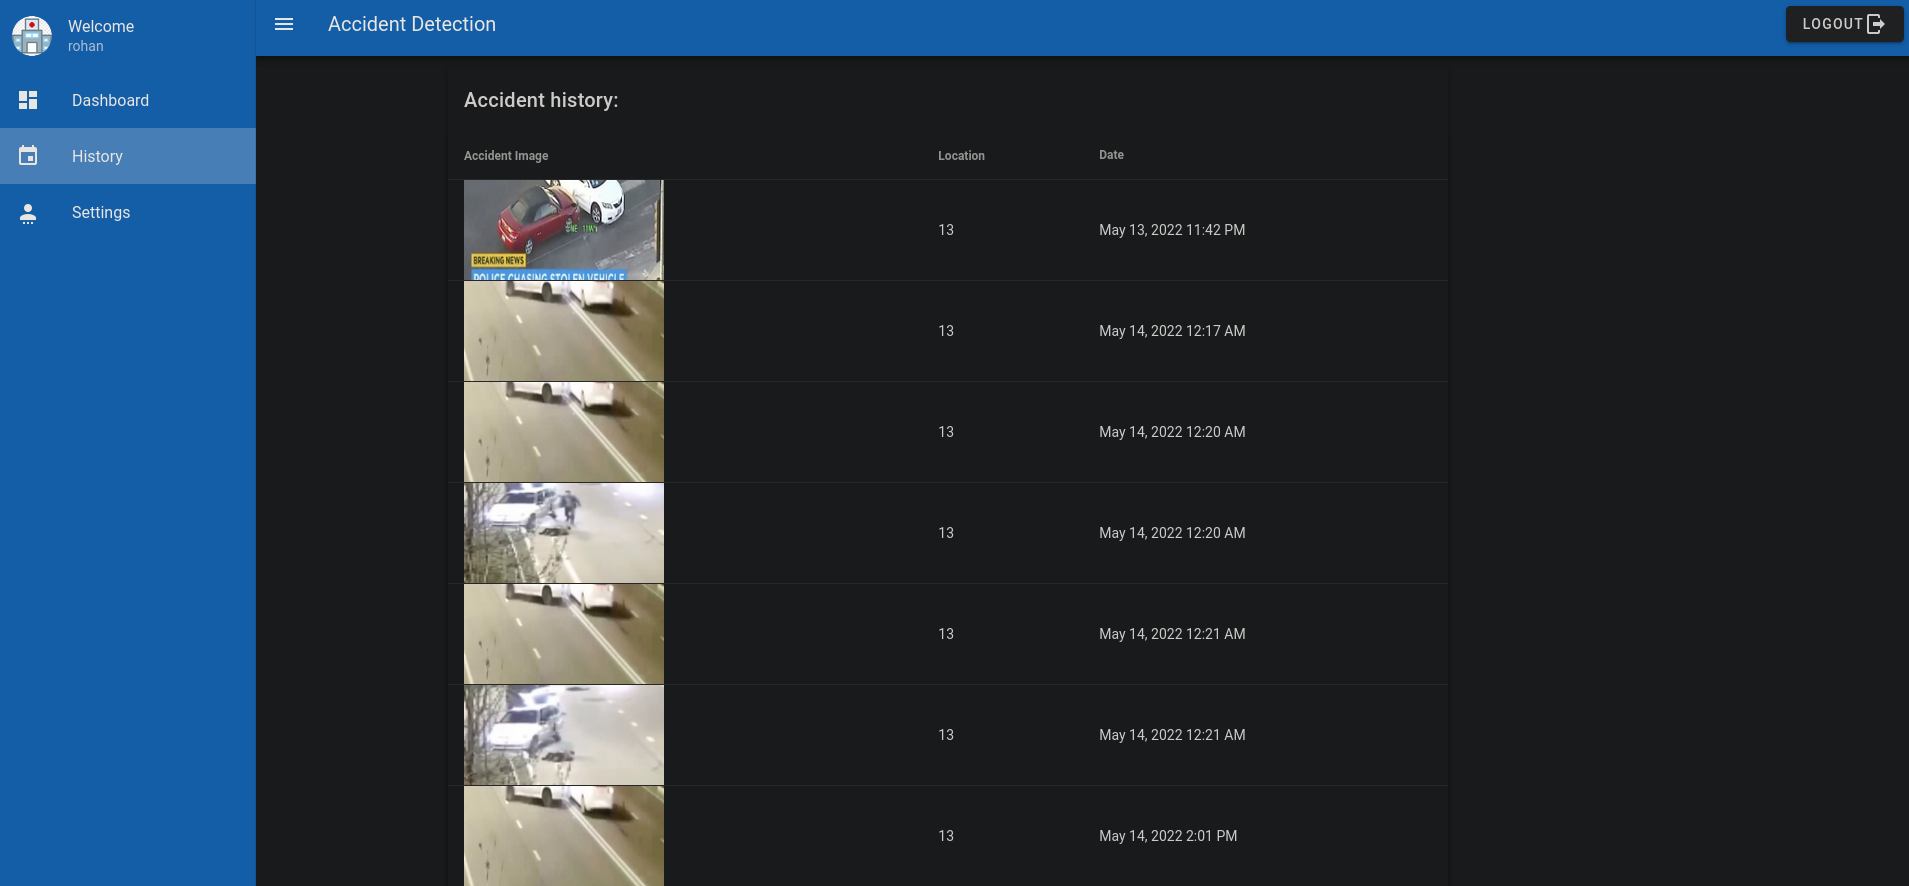
\includegraphics[scale=0.2]{media/ui2.png}
    \\
  \caption{ History of Accidents }
    
\end{center}
\end{figure}

\begin{figure}[H]
\begin{center}
    \hspace{0.2cm}
    
    \hspace*{0.4in}
    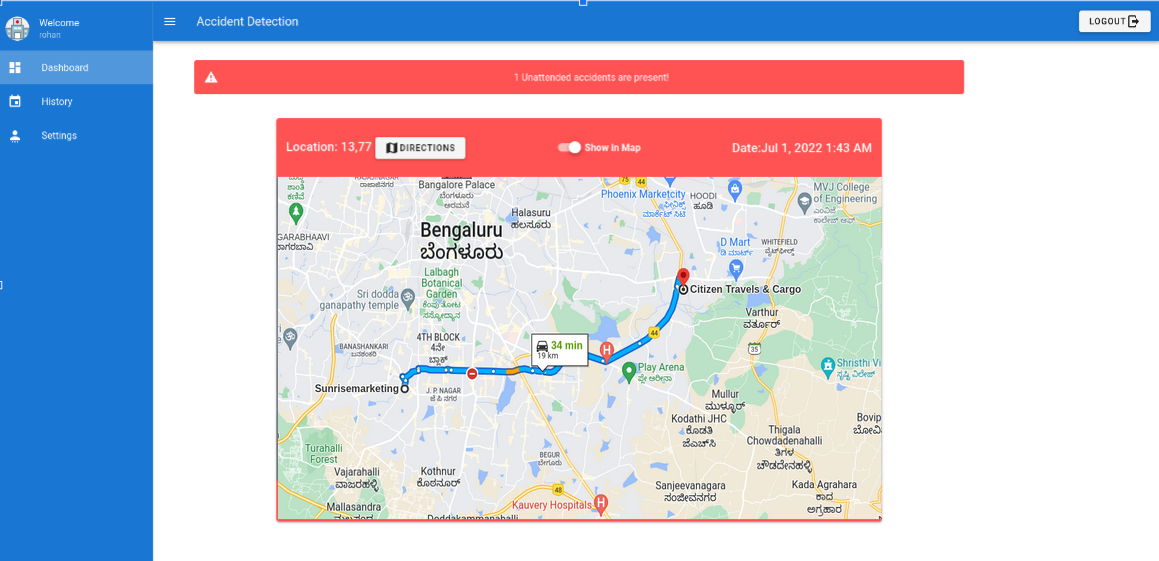
\includegraphics[scale=0.3]{media/maps.png}
    \\
  \caption{ Directions using Google Maps API}
\end{center}
\end{figure}
\vfill 

\newpage
  \pagestyle{fancy}

\vspace*{\fill}
\begin{figure}[H]
\begin{center}
    \hspace*{0.4in}
    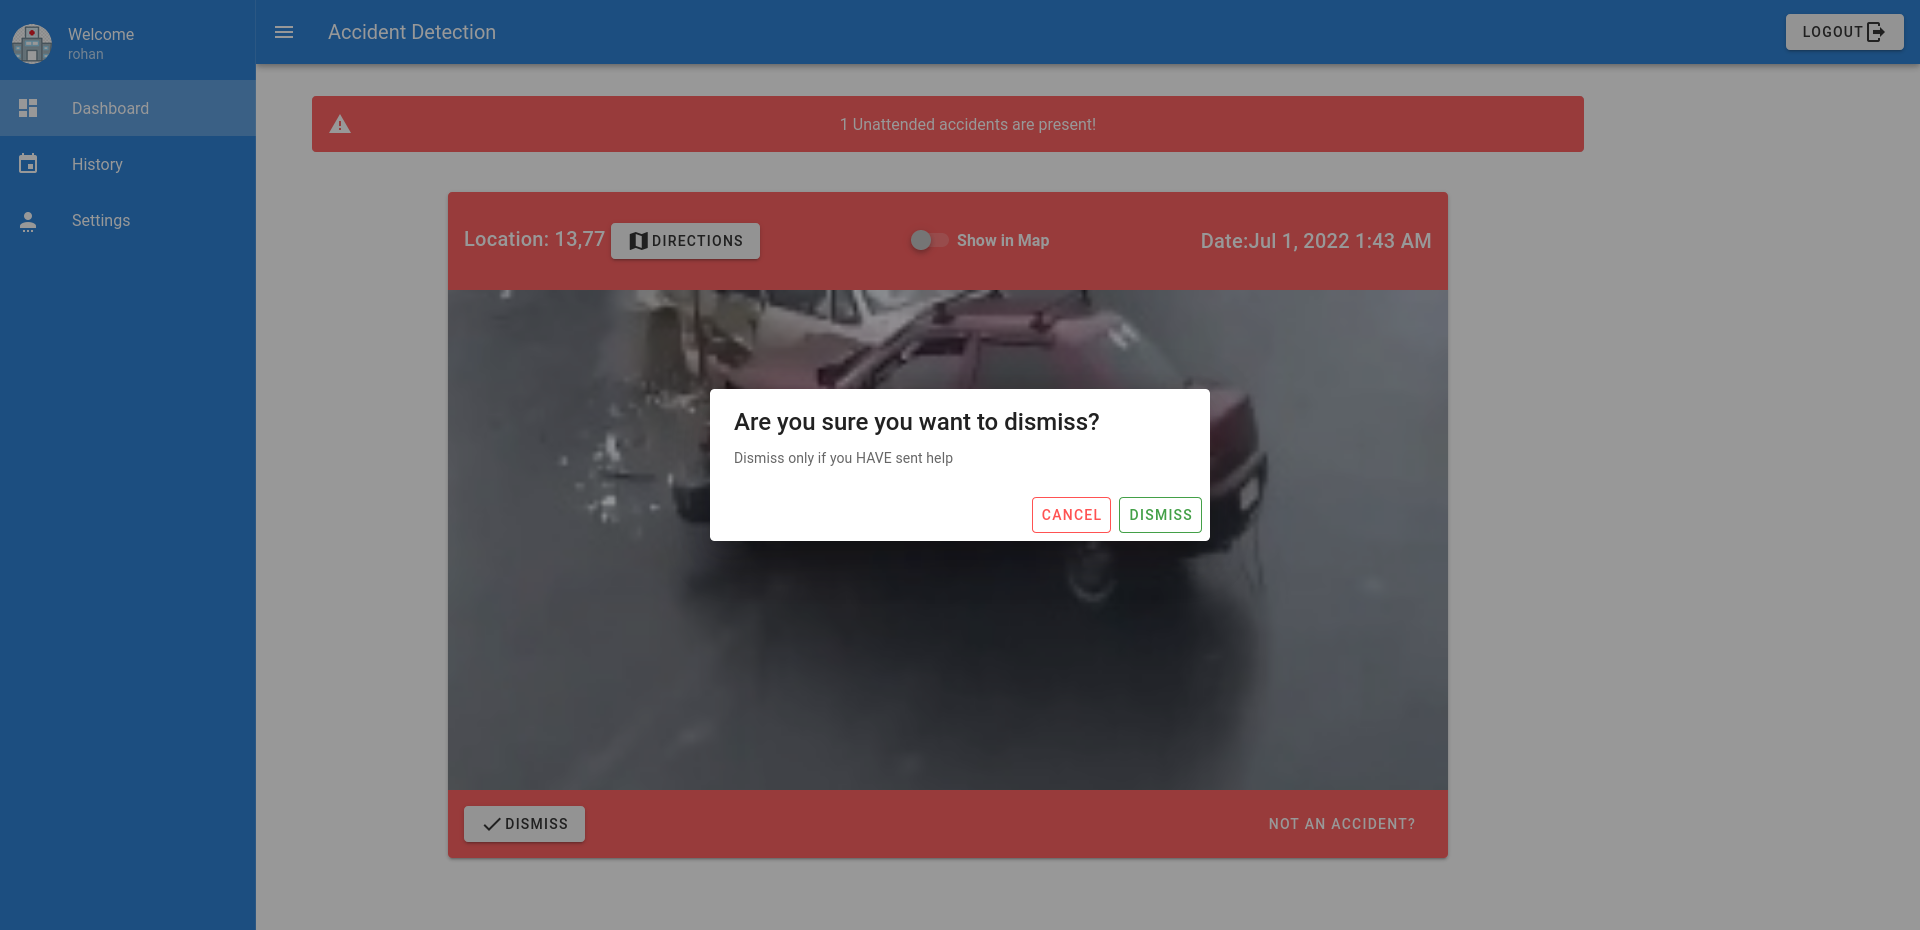
\includegraphics[scale=0.2]{media/dismiss.png}
    \\
  \caption{ Dismissing an Accident}
    
    \hspace{0.2cm}
\end{center}
\end{figure}

\begin{figure}[H]
\begin{center}
    \hspace*{0.4in}
    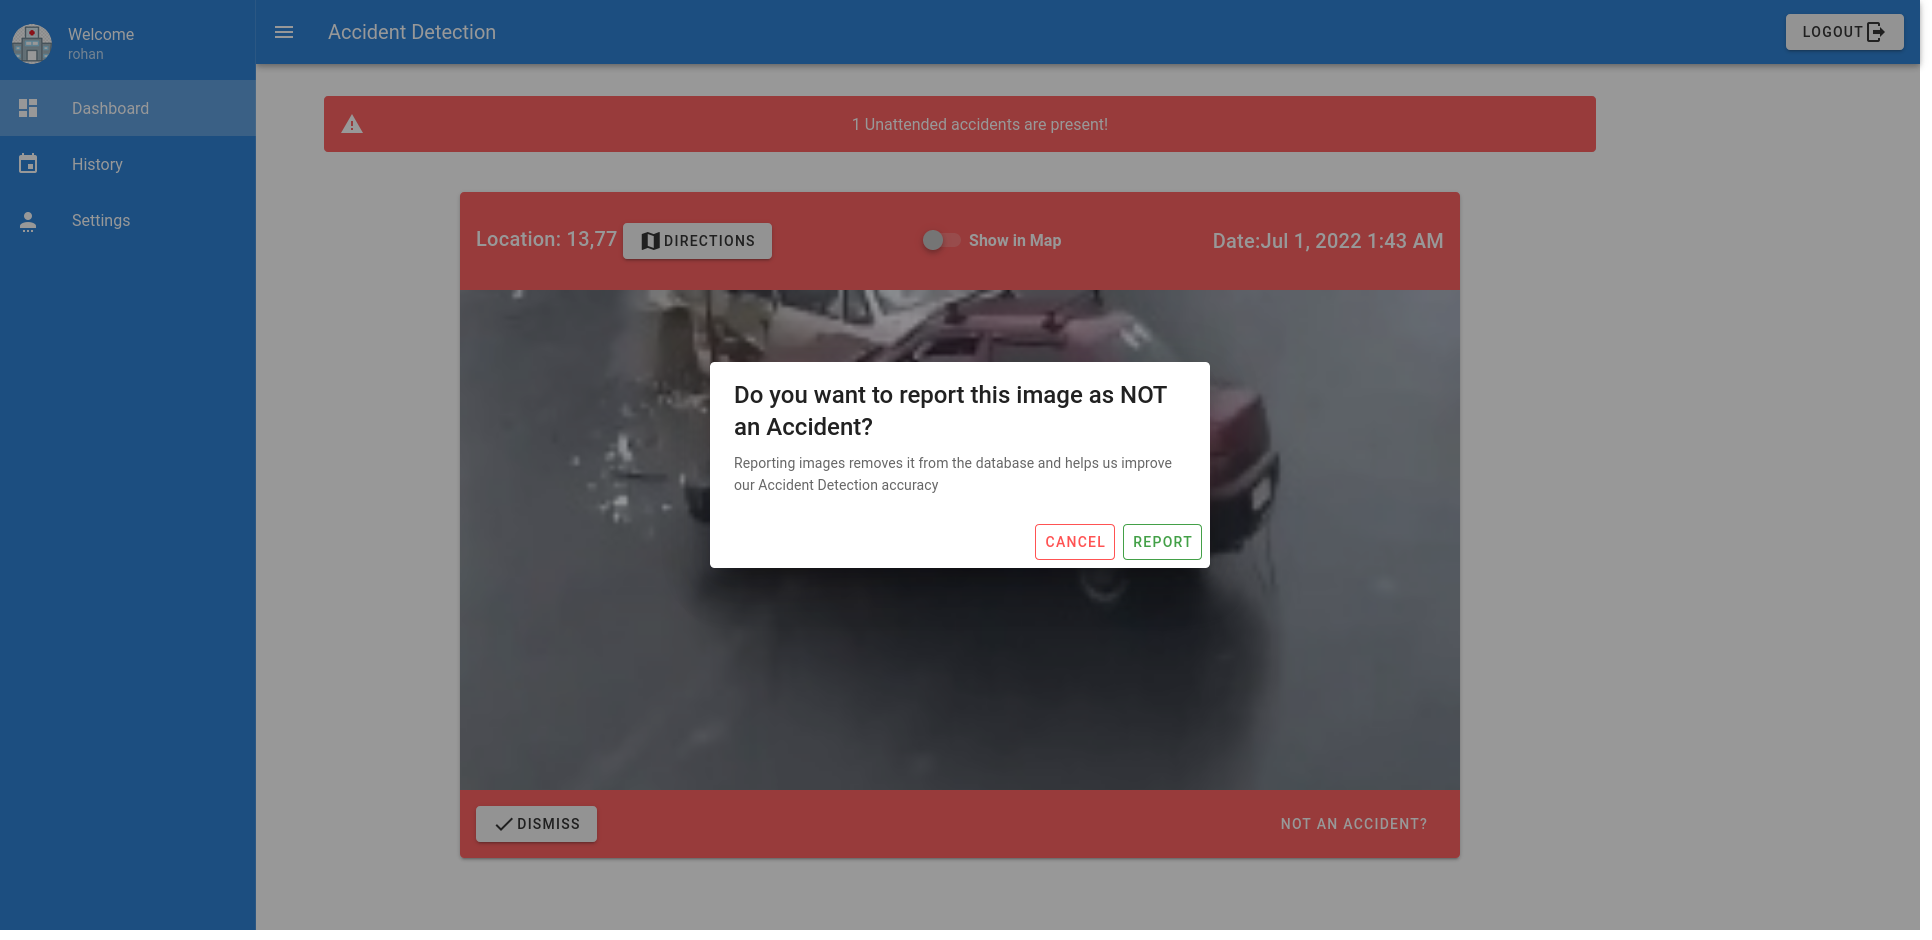
\includegraphics[scale=0.2]{media/report.png}
    \\
  \caption{ Reporting an Inaccurate Accident}
\end{center}
\end{figure}
\vfill 

\newpage
  \pagestyle{fancy}
  
\subsection{Dataset}

The Dataset forms the most important part of the project. Without a proper dataset covering various scenarios, we would not be able to build an efficient classifier that would accurately predict the occurrence of an accident.

Our dataset contains 5000 images divided into two classes: Accidents and Non-Accidents. The Accident class is made up of 2500 images of various types and angles of accidents. This data was extracted from CCTV Video footage uploaded to Youtube along with Google image results.
We experimented with simulated footage using Beam.NG, an extremely detailed and authentic vehicle simulation software. However, we felt that the simulated footage was not photo-realistic enough and did not complement the existing dataset well, so we chose to not use it. We also manually cleaned the Accident class, and removed images that did not belong to the class or was not good enough to be a part of the dataset.

The Non-Accident class is also made up of 2500 images, and mainly consists of various situations where vehicles are close to each other, and might appear to collide but are not. This class is crucial as it helps the model differentiate between cases where vehicles have actually collided and cases where the vehicles are close to each other but have not collided. This class ensures that the false positive alerts raised are kept in check.
    
\newpage

\vspace*{\fill}
\begin{figure}[H]
\begin{center}
    \hspace*{0.4in}
    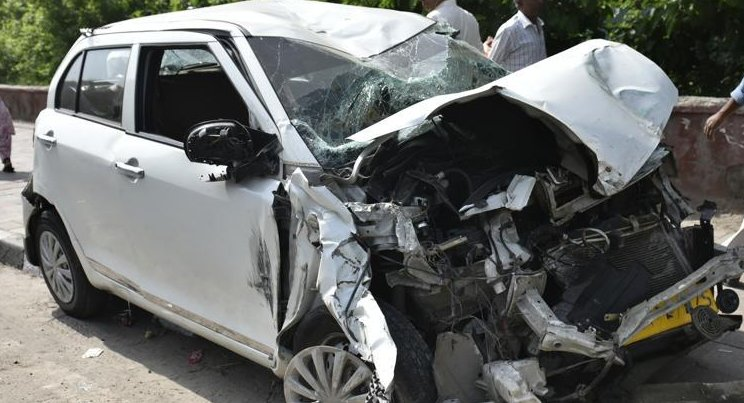
\includegraphics[scale=0.3]{media/acc1.jpg}
    
    \hspace{0.1cm}
\end{center}
\end{figure}
\begin{figure}[H]
\begin{center}
    
    \hspace*{0.4in}
    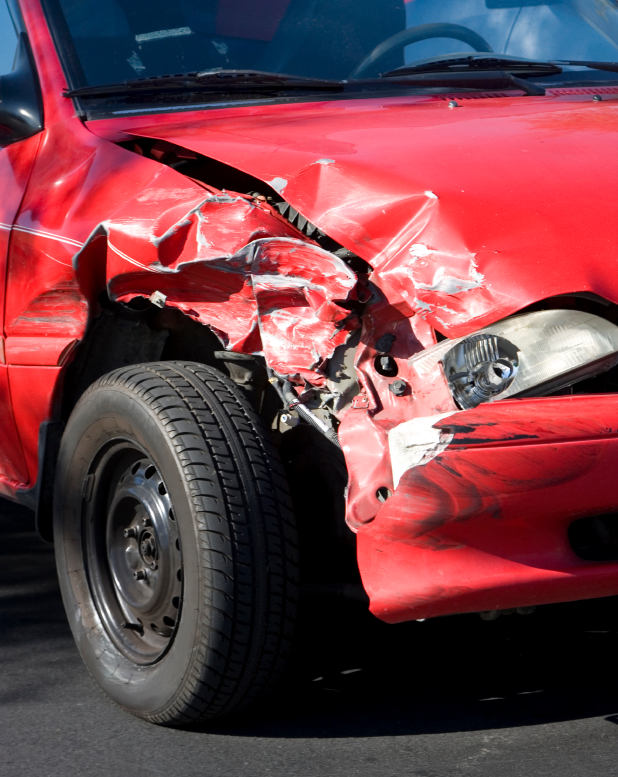
\includegraphics[scale=1]{media/acc2.jpg}
        
    \hspace{0.1cm}
\end{center}
\end{figure}
\begin{figure}[H]
\begin{center}
    
    \hspace*{0.4in}
    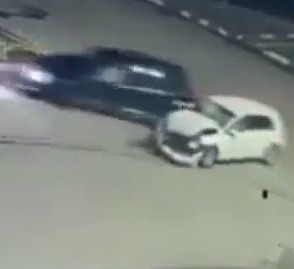
\includegraphics[scale=0.6]{media/acc3.jpg}
    
  \caption{ Example Dataset of Accident Class}
\end{center}
\end{figure}
\vfill

\newpage
  \pagestyle{fancy}

\vspace*{\fill}
\begin{figure}[H]
\begin{center}
    \hspace*{0.4in}
    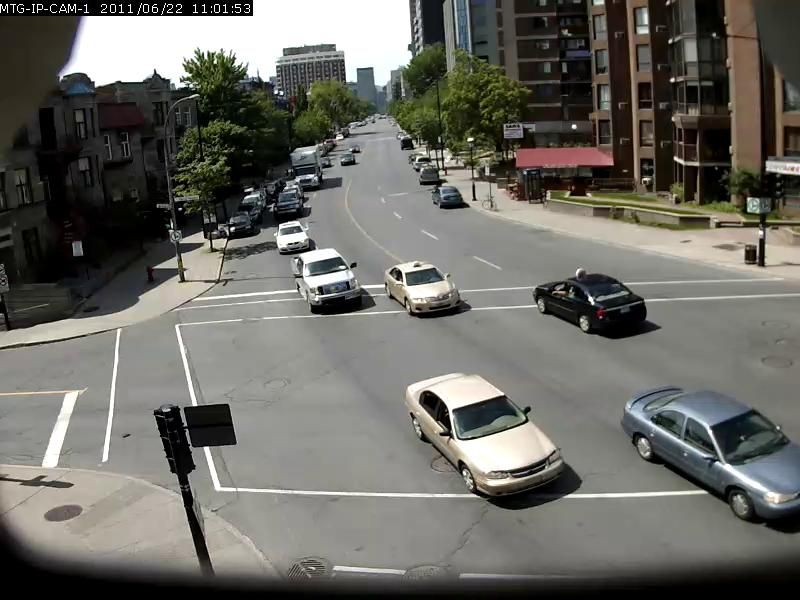
\includegraphics[scale=0.3]{media/noacc1.jpg}
        
    \hspace{0.1cm}
\end{center}
\end{figure}
\begin{figure}[H]
\begin{center}
    
    \hspace*{0.4in}
    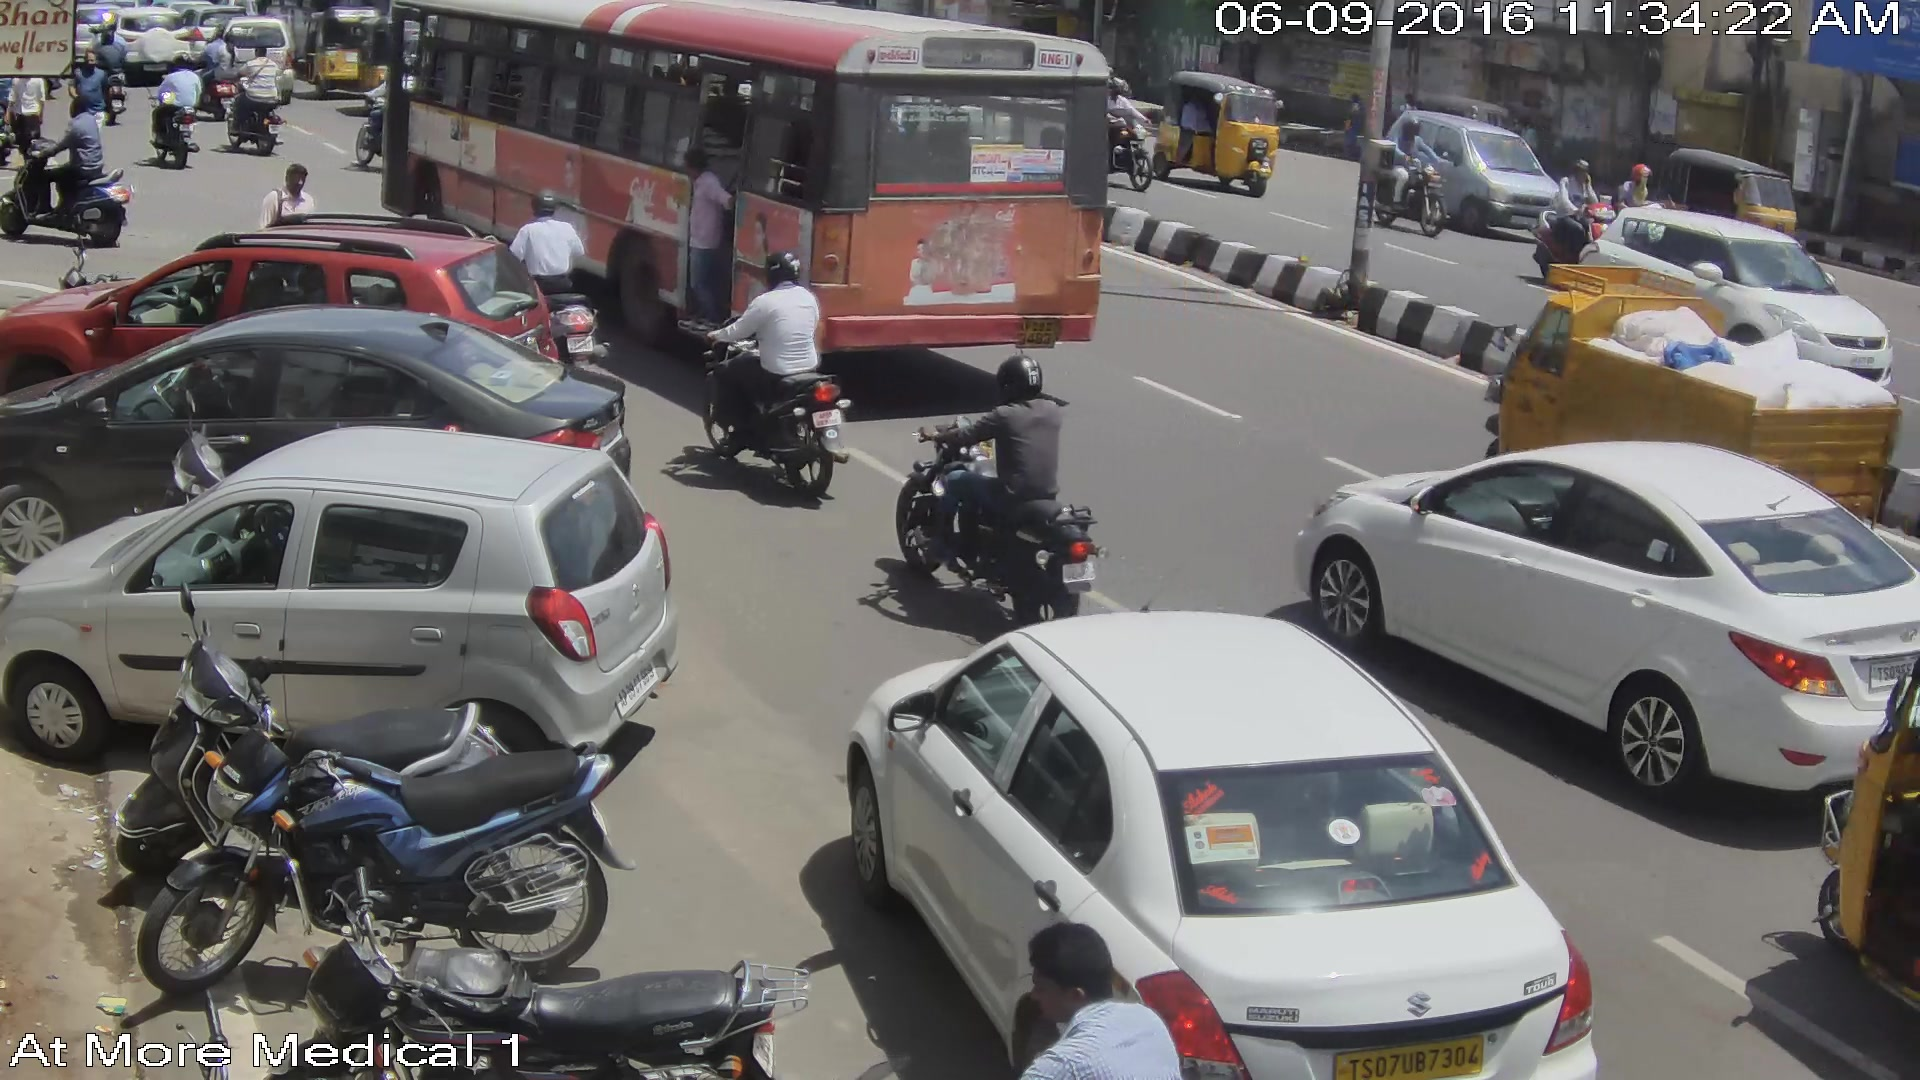
\includegraphics[scale=0.15]{media/noacc2.jpg}
        
    \hspace{0.1cm}
\end{center}
\end{figure}
\begin{figure}[H]
\begin{center}
    
    \hspace*{0.4in}
    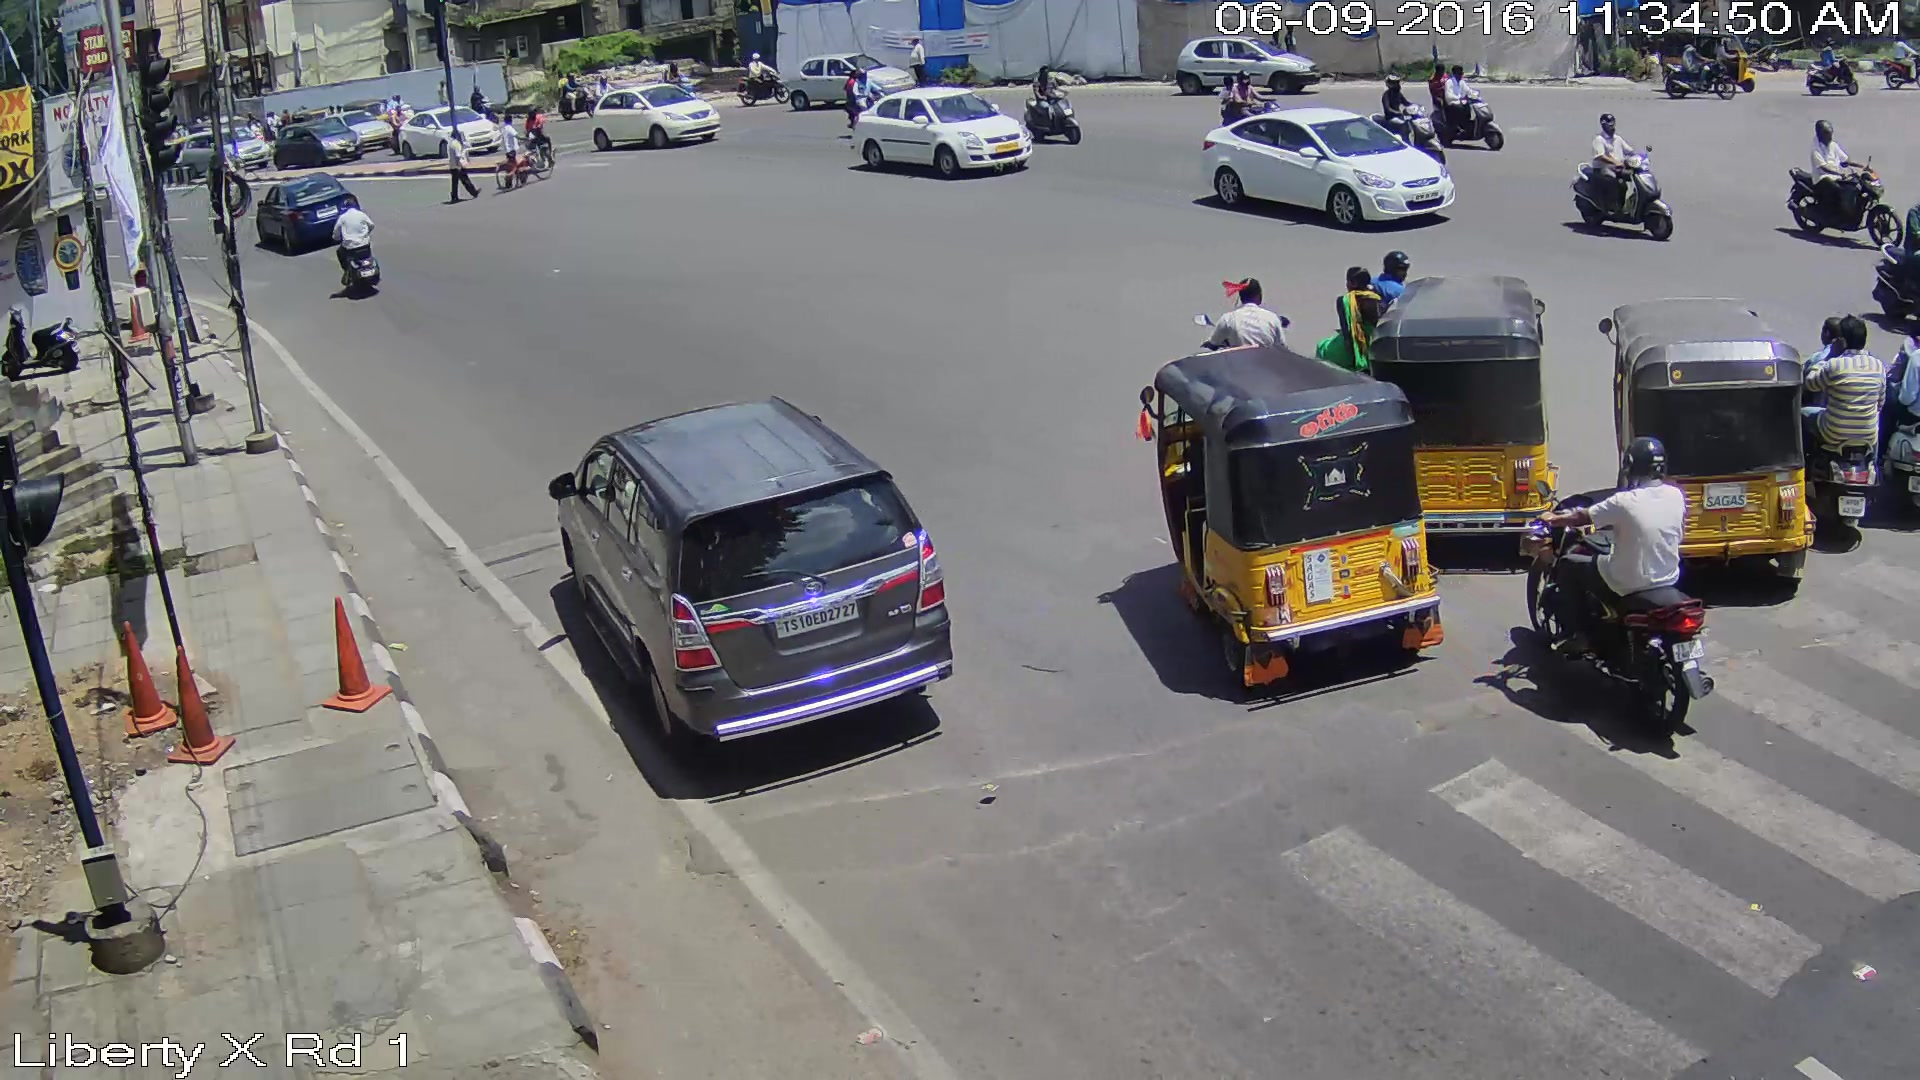
\includegraphics[scale=0.15]{media/noacc3.jpg}
    
  \caption{ Example Dataset of Non Accident Class}
\end{center}
\end{figure}
\vfill

\newpage
  \pagestyle{fancy}
  
\section{Testing}

The Deep Learning model’s performance was tested based on our initial dataset. The dataset consisted of ~2500 images each for both the classes (accident and not an accident). The dataset was split into train, test and evaluation data at 60\% for training, 20\% for testing and and the remaining 20\% for evaluation of the models performance.
This testing resulted in an accuracy of 97\% of the deep learning models in classification of accident images vs non-accident images.

In terms of end to end testing of the entire system involving the collision detection to the classification produced by the ANN, we used 15 videos of accidents gathered from the internet which provided an accurate estimate of the performance of the entire system.
A little more exploration was done through simulation of accidents where we used a Physics vehicular simulation software - Beam.NG Drive to gather footage of simulated accidents. 
The end to end testing provided an accuracy of 90\% with the collected videos where 5 of the videos were simulated ones and the other 15 were real-world accidents.

When measuring the latency or the time taken for the accident to be detected and reported, it was observed that the detection of accidents on a machine with appropriate hardware (8 gigabyte video memory along with 16 gigabyte memory) produced real-time results with an average of 45 frames per second.


\newpage
  \pagestyle{fancy}
  
\section{Experimentation and Results}

\subsection{Experimentation}

Extensive experimentation was carried out when working with this particular 2 stage accident detection system. When approaching the problem of object detection, various models were experimented with to compare and contrast between their accuracy and efficiency.
In terms of object detection as a whole, Single Stage detectors outperform all other methods of object detection and YOLO-v4 seems to outperform any other single stage detector.
Within yolo itself, there exist variations of the model for further fine tuning of accuracy and efficiency but the base YOLOv4 seemed to have a good balance between both of the metrics and we proceeded with this instead.

\hspace{0.2cm}

Collision Detection is a significant part of accident detection and we needed to ensure that the algorithm we chose would not lead to multiple false positives. As mentioned earlier, we made use of a variation of the Axis Aligned Bounding Box (AABB) method instead of the standard Intersection over Union (IOU) method. The reason for this is due to the relative position of the accident with respect to the CCTV camera footage. In the case where the accident is a distance away from the camera, the IOU method fails to take into consideration the actual percentage of overlap whereas the AABB method handles this effectively.

\newpage
  \pagestyle{fancy}
  
  \begin{figure}[H]
\begin{center}
    \hspace*{0.4in}
    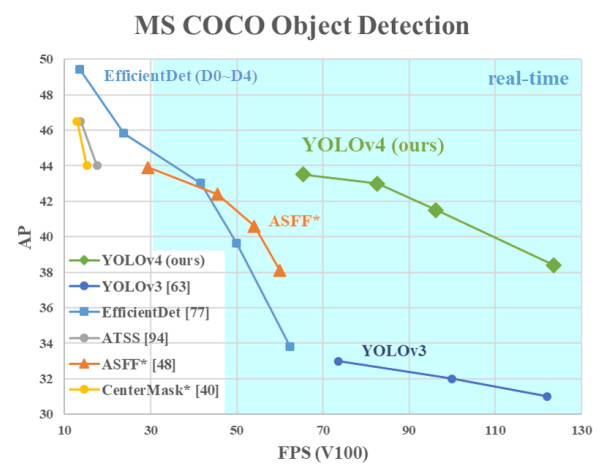
\includegraphics[scale=0.5]{media/res.png}
    \\
  \caption{ Performance of Yolov4 (Accuracy vs FPS)}
\end{center}
  \end{figure}


\hspace{0.2cm}
    
In the second stage of the system, from the view point of feature extraction, various methodologies such as Histogram of Gradients (HOG) and Canny edge detection. Older methods such as edge detection seemed to provide average results due it the edge detection being dependent on the surroundings of the accident, although many features of a car crash isn’t brought to context by Canny edge detection, it does extract useful information from the image and provide reasonable accuracy. Other feature detection algorithms such as Speeded Up Robust Features, Scale-Invariant feature transform have been tested with similar images and have been found to perform poorly in comparison to CNNs.
We make use of F1 score as a metric used for comparison. Accuracy is used when the True positives and true negatives are important whereas f1 score also takes into account the false positives and false negatives. In our use case, false negatives are to be minimised as every accident should be identified.
As mentioned earlier, we make use of a CNN for feature extraction combined with an ANN for classification. Experimentation was done with various models such as Resnet-50, Densenet, Inception-v3 and VGG16 all with a threshold probability score of 0.6.

\hspace{0.2cm}

When coming to the ANN that was used for classification, it consists of 3 hidden layers as shown in (link figure). The layers consist of 8, 32, and 16 neutrons respectively. In between each layer, there exists a dropout layer to prevent overfitting and a ReLU activation function as well. The final output layer consists of a single output neuron with a sigmoid activation function. The model was trained with a binary crosentrpoy loss and the Adam optimizer with a learning rate of 0.001 for 30 epochs and a batch size of 512 images.

\hspace{0.2cm}

\newpage
  \pagestyle{fancy}

\subsection{Results}

We evaluated the data against 20\% of the original dataset as evaluation data and the results are as shown in the table.

\begin{table}[H]
\centering
\footnotesize
\begin{tabular}{|p{4cm}| p{4cm}|}
\hline
CNN Architecture & F1-Score (N)\\
\hline\hline
Resnet-50 & 0.95 \\
Densenet-201 & 0.97 \\
Inception-v3 & 0.94 \\
VGG16 & 0.93 \\
\hline
\end{tabular}
\caption{F1 Score for each CNN Architecture}
\label{table:10}
\end{table}

\hspace{0.2cm}

From the results we see that the Densenet-201 architecture performs significantly better than the other CNNs for feature extraction, in the case of the end to end system, we trained the model on all of the images from our dataset and tested it on videos of accidents

\hspace{0.2cm}

\begin{figure}[H]
\begin{center}
    \hspace*{0.4in}
    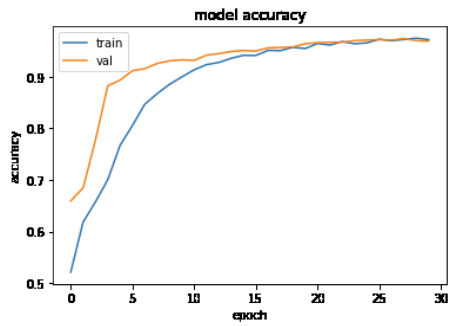
\includegraphics[scale=0.7]{media/acc.png}
    \\
  \caption{ Train vs Test Accuracy}
\end{center}
\end{figure}

\hspace{0.2cm}

\begin{figure}[H]
\begin{center}
    \hspace*{0.4in}
    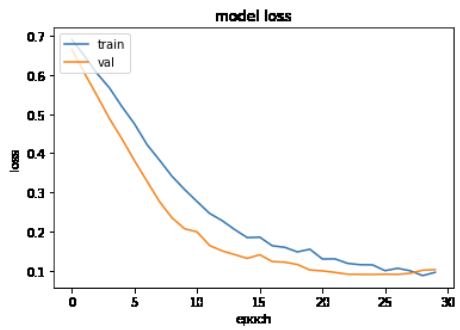
\includegraphics[scale=0.7]{media/loss.png}
    \\
  \caption{ Train vs Test Loss}
\end{center}
\end{figure}

\newpage
    \pagestyle{fancy}
    
\section{Conclusion}

With the ever increasing number of road accidents and fatalities of these accidents, an efficient accident detection and reporting is the need of the hour. The goal of our project was to create an accurate end to end system, utilizing the existing CCTV camera network infrastructure along with our processing framework and an end user web-based portal to display the report of the accident. For the same, we came up with a five stage process, starting with the frames being extracted from the video, to the application of YOLO for objection detection, our custom collision detection algorithm and our self-trained classifier to classify the images as accidents or non accidents, to finally displaying the results of the classification process to a web platform that would be made available to emergency care centers, hospitals and police stations in the vicinity of the accident.

\hspace{0.2cm}


Our testing revealed several positives, with our framework accurately detecting accidents in 90\% of the test video set. Our model was also highly accurate, delivering an f1 score of 0.97.
Even with these promising results, there is a lot of scope for future improvement. Work can be done on the foundations we have laid out to ensure the creation of a truly state of the art system. Some of the improvements that can be made are:

\begin{itemize}
    \item Improved accuracy of the model with the help of better, more varied datasets to cut down false positives.
    \item Estimation of Distance to the closest emergency response center to avoid redundancy.
    \item Partnerships with companies to create a joint platform for accident response.
    \item Better image processing to detect accidents in bad weather.
    \item Utilize incorrectly classified accidents and correct predictions to retrain the model in real time ensuring optimal performance.
    \item Addition of Automatic Number Plate Recognition to retrieve details of those involved in the incident.
\end{itemize}
% \newpage
%     \pagestyle{fancy}

%
% ---- Bibliography ----
%
% BibTeX users should specify bibliography style 'splncs04'.
% References will then be sorted and formatted in the correct style.
%
% \bibliographystyle{splncs04}
% \bibliography{mybibliography}
%
\begin{thebibliography}{8}
\bibitem{b1} Mathew, Reuben and Paul, Jeffery and Jamadagni, Rohan and Shruthii, RG and Malagi, Vindhya, A Comprehensive Study on Hardware and Software Based Accident Detection Systems (April 28, 2022). Available at SSRN: https://ssrn.com/abstract=4096390 or http://dx.doi.org/10.2139/ssrn.4096390
\bibitem{b2} Sánchez-Mangas, R., A. García-Ferrrer, A. De Juan and A. M. Arroyo. The Probability of   Death in Road Traffic Accidents. How Important Is a Quick Medical Response? Accident Analysis \& Prevention, Vol. 42, No. 4, 2010, pp. 1048-1056.
\bibitem{b3} Bansal, Prateek \& Kockelman, Kara \& Schievelbein, Will \& Schauer-West, Scott. (2018). Indian vehicle ownership and travel behavior: A case study of Bengaluru, Delhi and Kolkata. Research in Transportation Economics. 71. 10.1016/j.retrec.2018.07.025.
\bibitem{b4} Lee, J., Abdel-Aty, M., Cai, Q., \& Wang, L. (2018). Analysis of Fatal Traffic Crash-Reporting and Reporting-Arrival Time Intervals of Emergency Medical Services. Transportation Research Record, 2672(32), 61–71.
\bibitem{b5}R. N. Nayan Kumar, V. R. Navya, N. Ganashree, K. U. Pranav, and N. Ajay, ‘‘Intelligent vehicle accident detection and ambulance rescue system,’’ Int. J. Advance Res., Ideas Innov. Technol., vol. 5, no. 3, pp. 685–687, 2019.
\bibitem{b6} Manuja M et. al., (2019). Iot Based Automatic Accident
Detection And Rescue Management In Vanet. SSRG
International Journal of Computer Science and Engineering
(SSRG – IJCSE ), ISSN: 2348 – 8387.Pp. 36-41.
\bibitem{b7} Bansal, B. and Garg, V. (2019). Development of Message
Queuing Telemetry Transport (MQTT) based Vehicle
Accident Notification System.International Journal of
Engineering and Advanced Technology (IJEAT) ISSN: 2249 –
8958, Volume-9 Issue-2.pp. 268-273.
\bibitem{b8}L. Chuan-zhi, H. Ru-fu, Y.E. Hong-wu, “Method of Freeway Incident Detection Using wireless Positioning,” in Proceedings of the IEEE International Conference on Automation and Logistics, 2008, pp. 2801 - 2804.
\bibitem{b9}M. Syedul Amin, J. Jalil, and M. B. I. Reaz, ‘‘Accident detection and reporting system using GPS, GPRS and GSM technology,’’ in Proc. Int.Conf. Informat., Electron. Vis. (ICIEV), May 2012, pp. 640–643.
\bibitem{10}M. Murshed and M. S. Chowdhury, "An IoT based car accident prevention and detection system with smart brake control", Proc. Int. Conf. Appl. Techn. Inf. Sci. (iCATIS), pp. 23, 2019.
\bibitem{11}M. A. Khan and S. F. Khan, "IoT based framework for Vehicle Over-speed detection," 2018 1st International Conference on Computer Applications \& Information Security (ICCAIS), 2018, pp. 1-4, doi: 10.1109/CAIS.2018.8441951.
\bibitem{12}Reddy, V. et al., (2014). Design and Development of accelerometer based System for driver safety. International Journal of Science, Engineering and Technology Research (IJSETR), Volume 3, Issue 12, ISSN: 2278 – 7798.pp. 3463- 3468.
\bibitem{13}Bergonda, S., et. al. (2017, April). “IoT Based Vehicle
Accident Detection and Tracking System Using GPS Modem”,
International Journal of Innovative Science and Research
Technology(IJISRT) ISSN No: - 2456 – 2165, Volume 2, Issue
4.
\bibitem{14}A. T. Mohammed and N. A. Kamsani, "Automatic accident detector and reporting system (Hardware and software) ECBA medical system," 2017 IEEE 15th Student Conference on Research and Development (SCOReD), 2017, pp. 35-38, doi: 10.1109/SCORED.2017.8305425.
\bibitem{15}Sri Krishna Chaitanya Varma, Poornesh, Tarun Varma, Harsha; Automatic
Vehicle Accident Detection And Messaging System Using GPS and GSM
Modems; International Journal of Scientific \& Engineering Research,
Volume 4, Issue 8, August-2013.
\bibitem{16}Robles-Serrano, S.; Sanchez-Torres, G.; Branch-Bedoya, J. Automatic Detection of Traffic Accidents from Video Using Deep Learning Techniques. Computers 2021, 10, 148.
\bibitem{17}A. Krizhevsky, I. Sutskever, and G. E. Hinton, “ImageNet classification with deep convolutional Neural Networks,” Communications of the ACM, vol. 60, no. 6, pp. 84–90, 2017.
\bibitem{18}S. Ghosh, S. J. Sunny and R. Roney, "Accident Detection Using Convolutional Neural Networks," 2019 International Conference on Data Science and Communication (IconDSC), 2019, pp. 1-6, doi: 10.1109/IconDSC.2019.8816881.
\bibitem{19}Bochkovskiy, Alexey \& Wang, Chien-Yao \& Liao, Hong-yuan. (2020). YOLOv4: Optimal Speed and Accuracy of Object Detection
\bibitem{20}D. Chand, S. Gupta, and I. Kavati, “Computer Vision based accident detection for Autonomous Vehicles,” 2020 IEEE 17th India Council International Conference (INDICON), 2020.
\bibitem{21}E. P. Ijjina, D. Chand, S. Gupta and K. Goutham, "Computer Visionbased Accident Detection in Traffic Surveillance," 2019 10th International Conference on Computing, Communication and Networking Technologies (ICCCNT), 2019, pp. 1-6, doi: 10.1109/ICCCNT45670.2019.8944469.
\bibitem{22}Chen Wang, Yulu Dai, Wei Zhou, Yifei Geng, "A Vision-Based Video Crash Detection Framework for Mixed Traffic Flow Environment Considering Low-Visibility Condition", Journal of Advanced Transportation, vol. 2020, Article ID 9194028, 11 pages, 2020.
\bibitem{23}W. Huang, G. Peng, and X. Tang, “A limit of densely connected convolutional networks V1,” protocols.io, 2019.
\bibitem{24}K. Dwivedi, K. Biswaranjan, and A. Sethi, ‘‘Drowsy driver detection
using representation learning,’’ in Proc. IEEE Int. Advance Comput. Conf.
(IACC), Feb. 2014, pp. 995–999.
\bibitem{25}O. G. Basubeit, D. N. T. How, Y. C. Hou, and K. S. M. Sahari, ‘‘Distracted
driver detection with deep convolutional neural network,’’ Int. J. Recent
Technol. Eng., vol. 8, no. 4, pp. 6159–6163, 2019.
\bibitem{26}M. Szarvas, A. Yoshizawa, M. Yamamoto, and J. Ogata, ‘‘Pedestrian detec-
tion with convolutional neural networks,’’ in Proc. IEEE Intell. Vehicles
Symp., Las Vegas, NV, USA, Jun. 2005, pp. 224–229.
\bibitem{27}Pashaei, Ali \& Ghatee, Mehdi \& Sajedi, Hedieh. (2020). Convolution neural network joint with mixture of extreme learning machines for feature extraction and classification of accident images. Journal of RealTime Image Processing.
\bibitem{28}Kodali, R. and Sahu, S. (2017). MQTT Based Vehicle Accident Detection and Alert System.International Conference on Applied and Theoretical Computing and Communication Technology
\bibitem{29}W. Farooq, M. A. Khan, S. Rehman, and N. A. Saqib, "A survey of multicast routing protocols for vehicular ad hoc networks," Int. J. Distrib. Sensor Netw., vol. 11, no. 8, 2015, Art. no. 923086.
\bibitem{30}Z. Cao, K. Shi, Q. Song and J. Wang, "Analysis of correlation between vehicle density and network congestion in VANETs," 2017 7th IEEE International Conference on Electronics Information and Emergency Communication (ICEIEC), 2017, pp. 409-412, doi: 10.1109/ICEIEC.2017.8076593.
\bibitem{31}B. Shabir, M. A. Khan, A. U. Rahman, A. W. Malik, and A. Wahid, "Congestion avoidance in vehicular networks: A contemporary survey," IEEE Access, vol. 7, pp. 173196–173215, 2019.
\bibitem{32}B. Government of India Ministry of Road Transport and Highways Transport Research Wing "ROAD ACCIDENTS IN INDIA – 2018" [Online] Available: \url{https://morth.nic.in/sites/default/files/Road_Accidednts.pdf}
\end{thebibliography}

\end{adjustwidth}
\end{document}
